%% This is an example first chapter.  You should put chapter/appendix that you
%% write into a separate file, and add a line \include{yourfilename} to
%% main.tex, where `yourfilename.tex' is the name of the chapter/appendix file.
%% You can process specific files by typing their names in at the 
%% \files=
%% prompt when you run the file main.tex through LaTeX.
\chapter{Simulation Results}

This chapter focuses on the results of fault classification simulations under two main sections: classification of faults based on simulated flight measurements and classification of faults based on real flight data. 
In the first part, flight data simulation uses the mathematical equations explained under mathematical modeling chapter of this thesis. 
The second part starts with the explanations on the path to generate faults in real flight thoroughly for two reasons, the importance of having knowledge on data, how it is generated/labeled, and also constructing a guide for researches to realize their own faulty flight campaigns. 
After that, classification for control surface stuck and loss of effectiveness faults have been investigated separately. 

\section{Fault detection from simulated flight data}

In this section, model of an aircraft is simulated in Matlab using the equations of motion given Equ.~\ref{eqn:compactEquOfMotion}. 
This drone model, will not be used for the design of FDD algorithms, but to generate data that will be used by the FDD algorithms. 
After the equations of motion of drone have been solved numerically, accelerometer and gyro measurements have been simulated based on the statistics of the sensors onboard. 
This part of the study uses the model of a MAKO drone to simulate the measurements while the real flights that will be explained in the forthcoming section uses a ZAGI drone.

For MAKO simulation, the stability and aerodynamic force coefficients are generated by AVL. The input vector can be written as $\bm{u}\left(t\right) \in {\rm I\!R} ^3 $
\begin{equation}
\bm{u}\left(t\right)= \begin{bmatrix} {\delta}_{a}\ {\delta}_{e}\ n \end{bmatrix}^{\rm T}
\end{equation}

Here $ \delta_{a}$ aileron deflection angle in degrees, $ \delta_{e}$ elevator deflection angle in degrees, $n$ engine speed in rev/s. 

When the actuators are healthy, actual control input signal will be equal to the given input signal. In case of a fault the actual signal can be modeled as

\begin{equation}
\bm{u}\left(t\right)= \bm{E}\bm{u}_c + u_f
\end{equation}

where $\bm{u}_c $ is the desired control signal, $E = diag(e_1, e_2, e_3)$ is the effectiveness of the actuators where $0 \leq e_i \leq 1 $ with $(i = 1, 2 ,3)$ and $u_f$ additive actuator fault. 
This model makes it possible to simulate all four types of actuator faults shown in Fig.~\ref{fig:actuatorFaults}.

\begin{figure}
\begin{center}
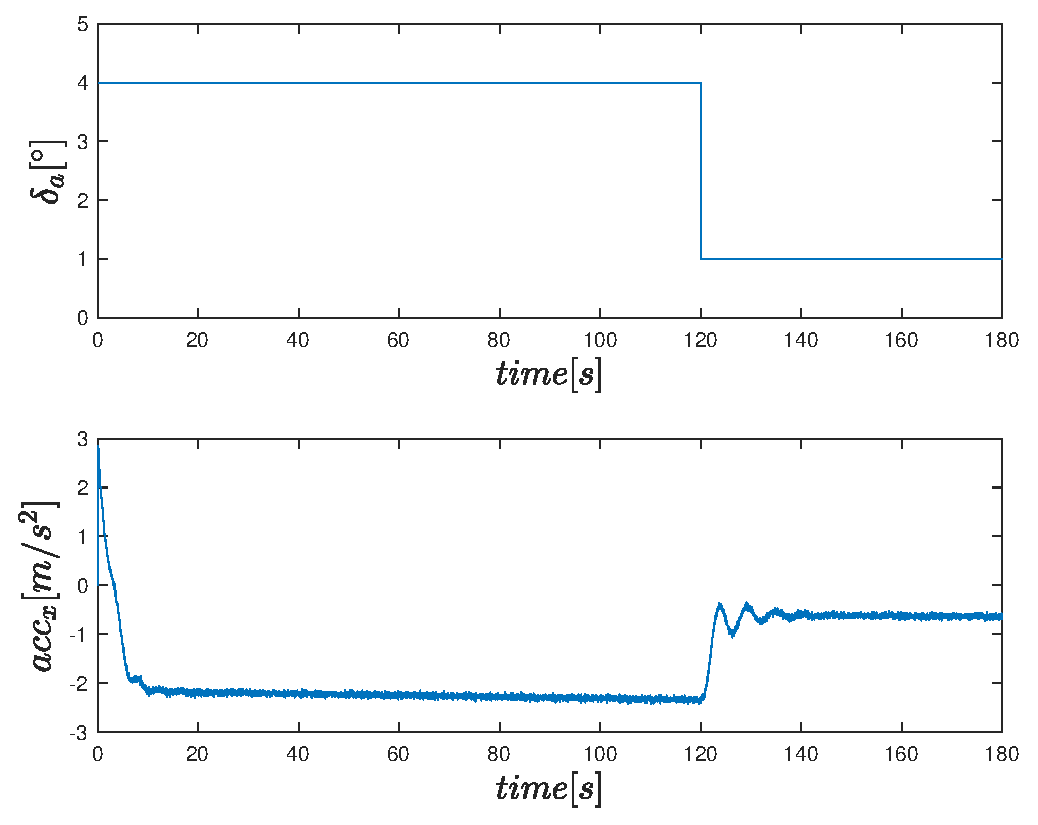
\includegraphics[width=12cm]{figures/control_input_acc_x}    % The printed column width is 8.4 cm.
\caption{Loss of effectiveness fault simulation in aileron command and corresponding accelerometer x axis measurement} 
\label{fig:faultSimulation}
\end{center}
\end{figure}

Most of the FDD algorithms are implemented to open-loop systems, ignoring the probable influences of the controller might cause on the detection performance \cite{pandita2013closed}. 
Throughout this first section, the system is open-loop as well.  
In this chapter, a step by step approach is followed. 
In this first section (diagnosis with simulated data) the effect of controller is ignored while in the next section (diagnosis with real flight data), diagnosis is achieved aside a functioning controller.

The code for simulations in this section can be reached in \emph{Github}\footnote{https://github.com/benelgiz/curedRone}. 
First, the measurements are simulated for faulty and nominal flight conditions. 
An example control input, 75\% loss of efficiency, could be an actual aileron command of $\delta_{a}^a=1^\circ$ corresponding to a desired $\delta_{a}^d=4^\circ$. In the simulation, this fault, is introduced after 120 s. Actual aileron command and corresponding simulated accelerometer $x-axis$ readings can be seen in Fig.~\ref{fig:faultSimulation}. 
The measurements are labeled, and an example plot showing simulated measurements in two-dimensional feature space, $a_x$ - $a_y$, is given as in Fig.~\ref{fig:feat1vsfeat2}. 

\begin{figure}
\begin{center}
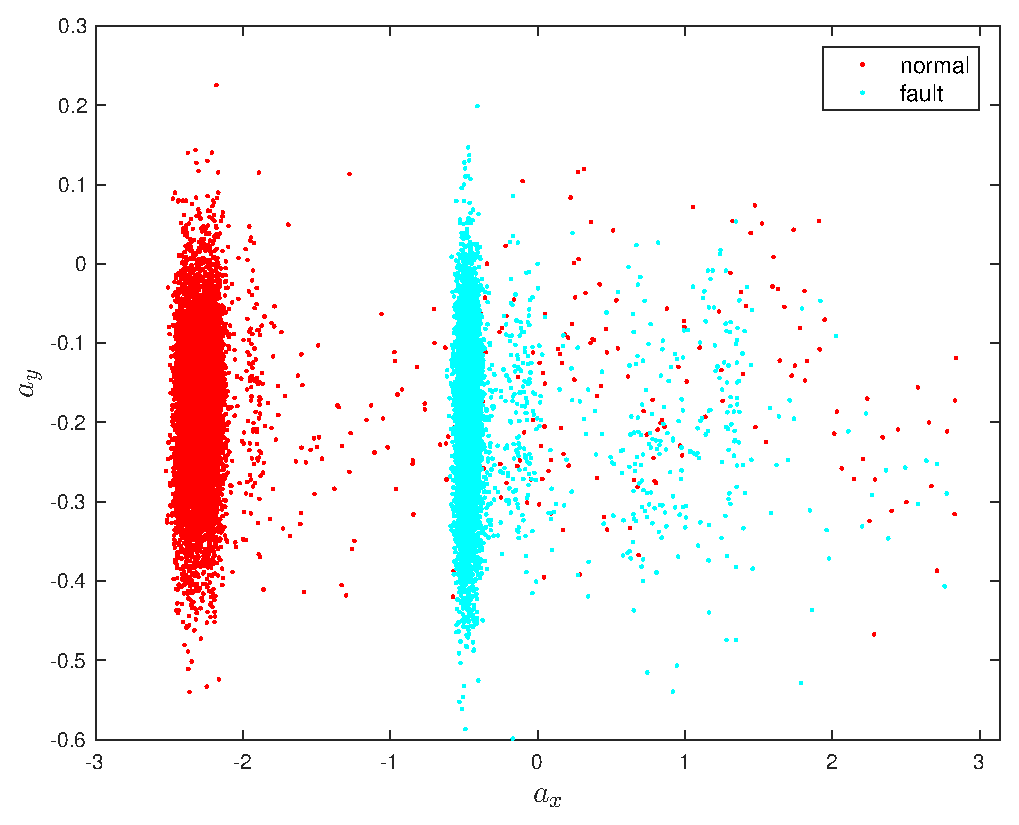
\includegraphics[width=12cm]{figures/feat1vsfeat2}    % The printed column width is 8.4 cm.
\caption{Accelerometer simulation $a_x$ vs $a_y$ } 
\label{fig:feat1vsfeat2}
\end{center}
\end{figure}

%\begin{figure}
%\begin{center}
%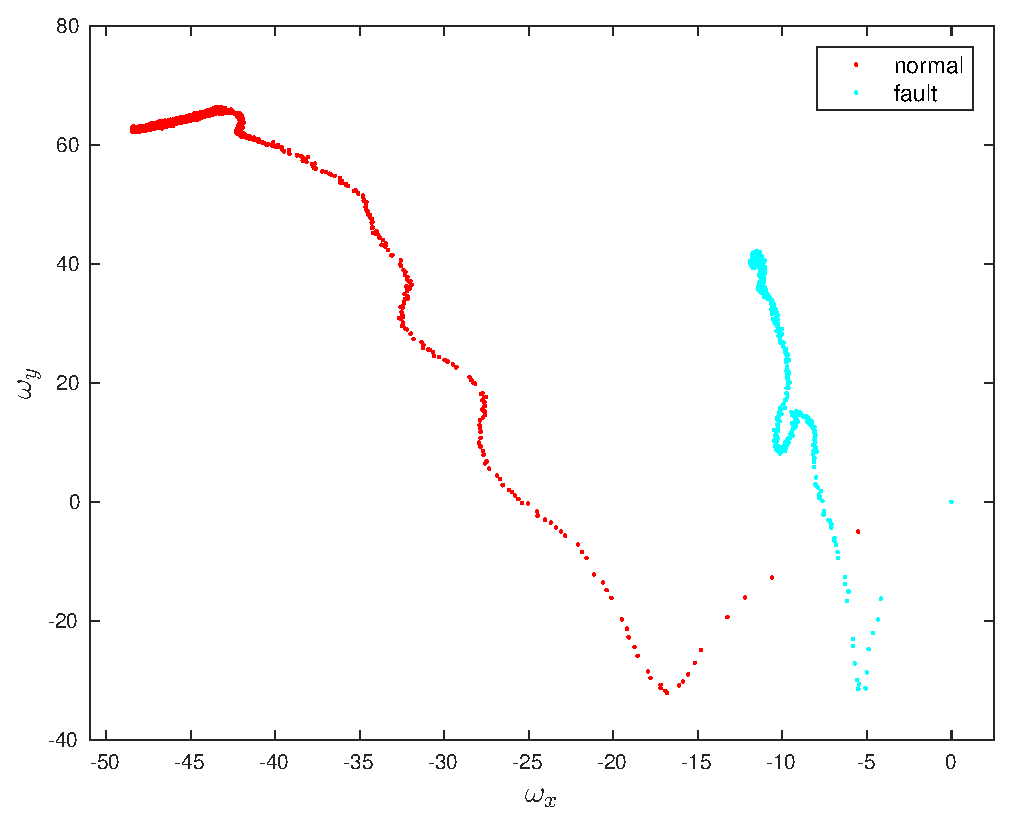
\includegraphics[width=12cm]{figures/feat4vsfeat5}    % The printed column width is 8.4 cm.
%\caption{Accelerometer simulation $a_x$ vs $a_y$ } 
%\label{fig:feat4vsfeat5}
%\end{center}
%\end{figure}

It is always important to visualize the features to have a grasp of data structure before applying machine learning algorithms. 
For that reason, available observations forms the 6-dimensional pattern space,  $\vec{\bm{x}} = \begin{bmatrix} {a_x} & {a_y} & {a_z} & {\omega_x} & {\omega_y} & {\omega_z}  \end{bmatrix}$ can be visualized in pairs such as Fig.~\ref{fig:feat1vsfeat2}. 
There are further methods to visualize multidimensional data such as \emph{Tours}\cite{asimov1985grand,cook1997manual,cook1995grand} and \emph{GGobi} data visualization system \cite{cook2007interactive}. In this work, dimensionality reduction technique, Principle Component Analysis (PCA), is utilized for visualization. If very briefly explained, the feature vector $\bm{x}\in{\rm I\!R}^{n}$ is mapped to a lower dimensional space where the 
new feature set will be represented by $\bm{z}\in{\rm I\!R}^{k}$. The final two dimensional feature set can be plotted to give an idea about faulty and nominal measurements' distribution in feature space as shown in Fig.~\ref{fig:z1_vs_z2}.

\begin{figure}
\begin{center}
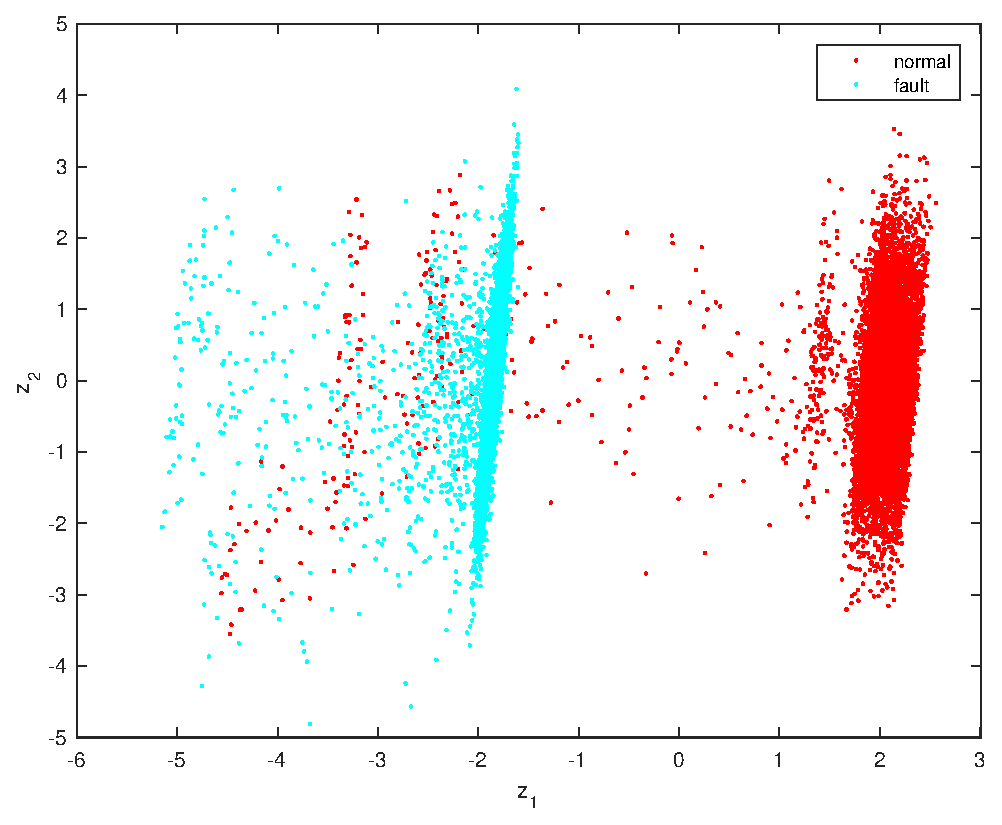
\includegraphics[width=12cm]{figures/reduceDimMeasurements}    % The printed column width is 8.4 cm.
\caption{Reduced dimensional space features $z_1$ vs $z_2$ } 
\label{fig:z1_vs_z2}
\end{center}
\end{figure}

\begin{figure}
\begin{center}
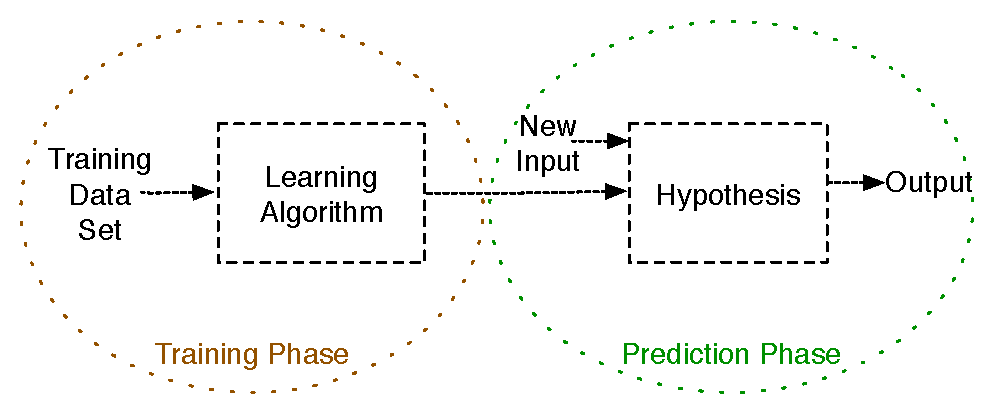
\includegraphics[width=12cm]{figures/supervisedLearningBasics}    % The printed column width is 8.4 cm.
% For the old picture 
% \includegraphics[width=12cm]{figures/machineLearningBasics}   
\caption{Supervised learning is achieved in two steps: \emph{Training Phase} in which the model parameters are calculated given labeled data and \emph{Prediction Phase} in which the label is predicted for a new input using the trained model.} 
\label{fig:supervisedLearning}
\end{center}
\end{figure}

The aim of machine learning methods is to train a model with a given data set in order to predict the output values corresponding to a new input.
A binary classifier is used in this work to classify two classes, faulty and nominal. 
The fault considered in this study is the loss of effectiveness of the control surfaces. 
SVM being a supervised classification algorithm has two main phases as shown in Fig.~\ref{fig:supervisedLearning}. 
In the training phase, the model is learned as a fit to the labeled data that is fed to the SVM algorithm. 
This phase is usually followed with a tuning phase where some of the parameters of SVM is changed and results are compared to have the best fit via cross validation to avoid overfitting. 
The last phase is the prediction, where for a new instance, the classifier predicts if it corresponds to a faulty or nominal condition.

Training data is comprised of labeled data where the label can belong to one of two possible cases. 
This data set is saved in $\bm{X} \in {\rm I\!R^{m \times n}}  $ where $m,n$ correspond to number of instances and features respectively (shown in Fig.~\ref{fig:featureMatrix}). 

\begin{figure}[h]
\begin{center}
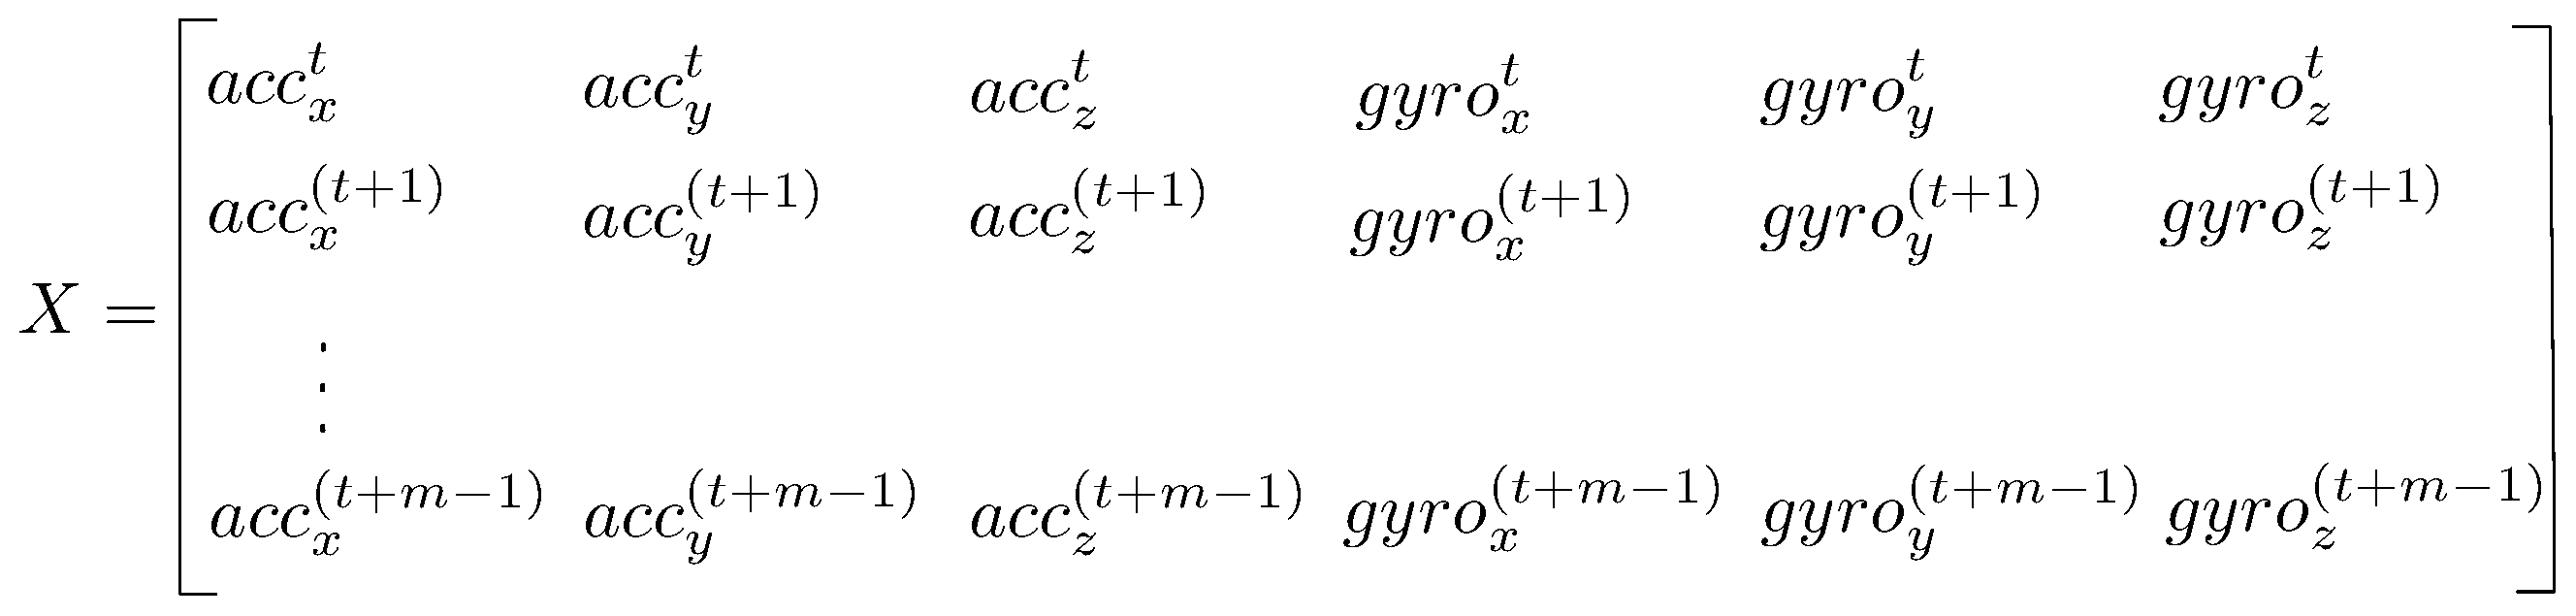
\includegraphics[width=13cm]{figures/featureMatrix}    % The printed column width is 8.4 cm.
\caption{Feature matrix $\bm{X} \in {\rm I\!R^{m \times 6}}  $  is comprised of accelerometer and gyro data of $m$ instances} 
\label{fig:featureMatrix}
\end{center}
\end{figure}

The label information corresponding to the measurement instances is also fed to the SVM algorithm during the training phase as output vector $\bm{y} \in \{-1,1\}$. 
The aim of SVM is to find an optimal hyperplane maximizing the margin by solving the optimization problem for non-linearly separable datasets. For further details on SVM and machine learning in general, the reader could refer to the methodology chapter of this thesis.

\begin{figure}
\begin{center}
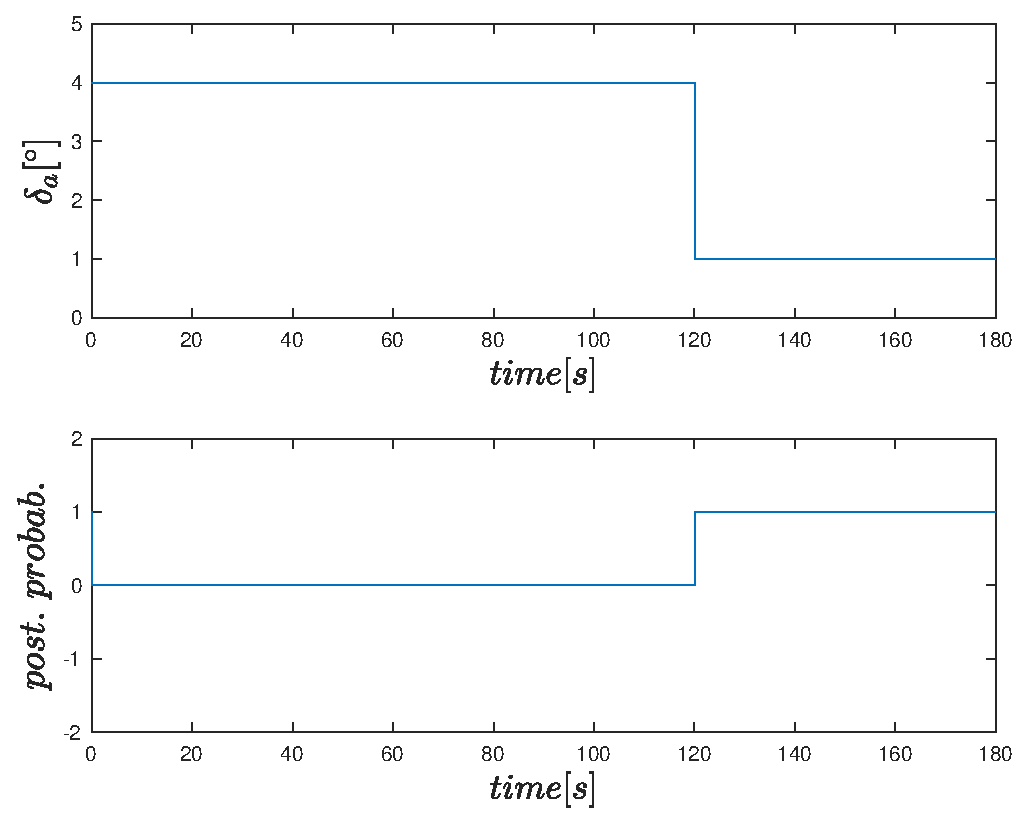
\includegraphics[width=11cm]{figures/post_prob}    % The printed column width is 8.4 cm.
\caption{Posterior probability of loss in effectiveness fault for test set when a fault is injected at t = 120s.} 
\label{fig:post_prob}
\end{center}
\end{figure}

To avoiding overfitting, which is the main problem of parametric discrimination approaches such as neural networks, parameter $C$ (box constraint) is tuned to result in the optimal fit for the cross validation set. Box constraint $C$ controls the values of the parameters learnt during the training phase, and further explained under methodology chapter.
The data set available is first divided into two portions with a percentage of \%20, \%80 where the bigger chunk is the training set and the remaining is the test set. 
Further, the training set is divided as cross-validation and training sets. 
The idea to split data is to avoid overfitting. 
Overfitting means that the models trained being very accurate fit for the data they are trained to but fail to generalize with new inputs resulting in bad prediction performance for the new data. 
To improve the performance of the classifier trained with, the training data, it is tuned with the cross validation data. 
And finally, ability of the classifier is tested on the test set. 
This parameter also tuned for the outliers to generalize the distribution of the data rather than resulting in fine fits for each individual data in the training set. 
With a satisfactory result of the training \& tuning is followed by the prediction where the classifier predicts if the new measurement data belongs to the faulty or nominal class. 
The output of the SVM classification is not the probability that the new measurement belongs to one class as is in the traditional classification problems, but directly the class information it belongs to. 
For investigating the performance of the classifier on the test set, a method \cite{platt1999probabilistic} is used to calculate the posterior probabilities giving the probability that the new measurements belongs to faulty mode. 
Results shows as in  Fig.~\ref{fig:post_prob} that proper tuning achieves very accurate and instant detection for the drone fault. 
   
%\begin{figure*}
%\begin{center}
%\includegraphics[width=14cm]{modelSelectionNonVisualizableData}    % The printed column width is 8.4 cm.
%\caption{Supervised learning basics } 
%\label{fig:supervisedLearning}
%\end{center}
%\end{figure*}

\begin{figure}
\begin{center}
%\includegraphics[width=17cm]{figures/paparazziControlModes}    % The printed column width is 8.4 cm.
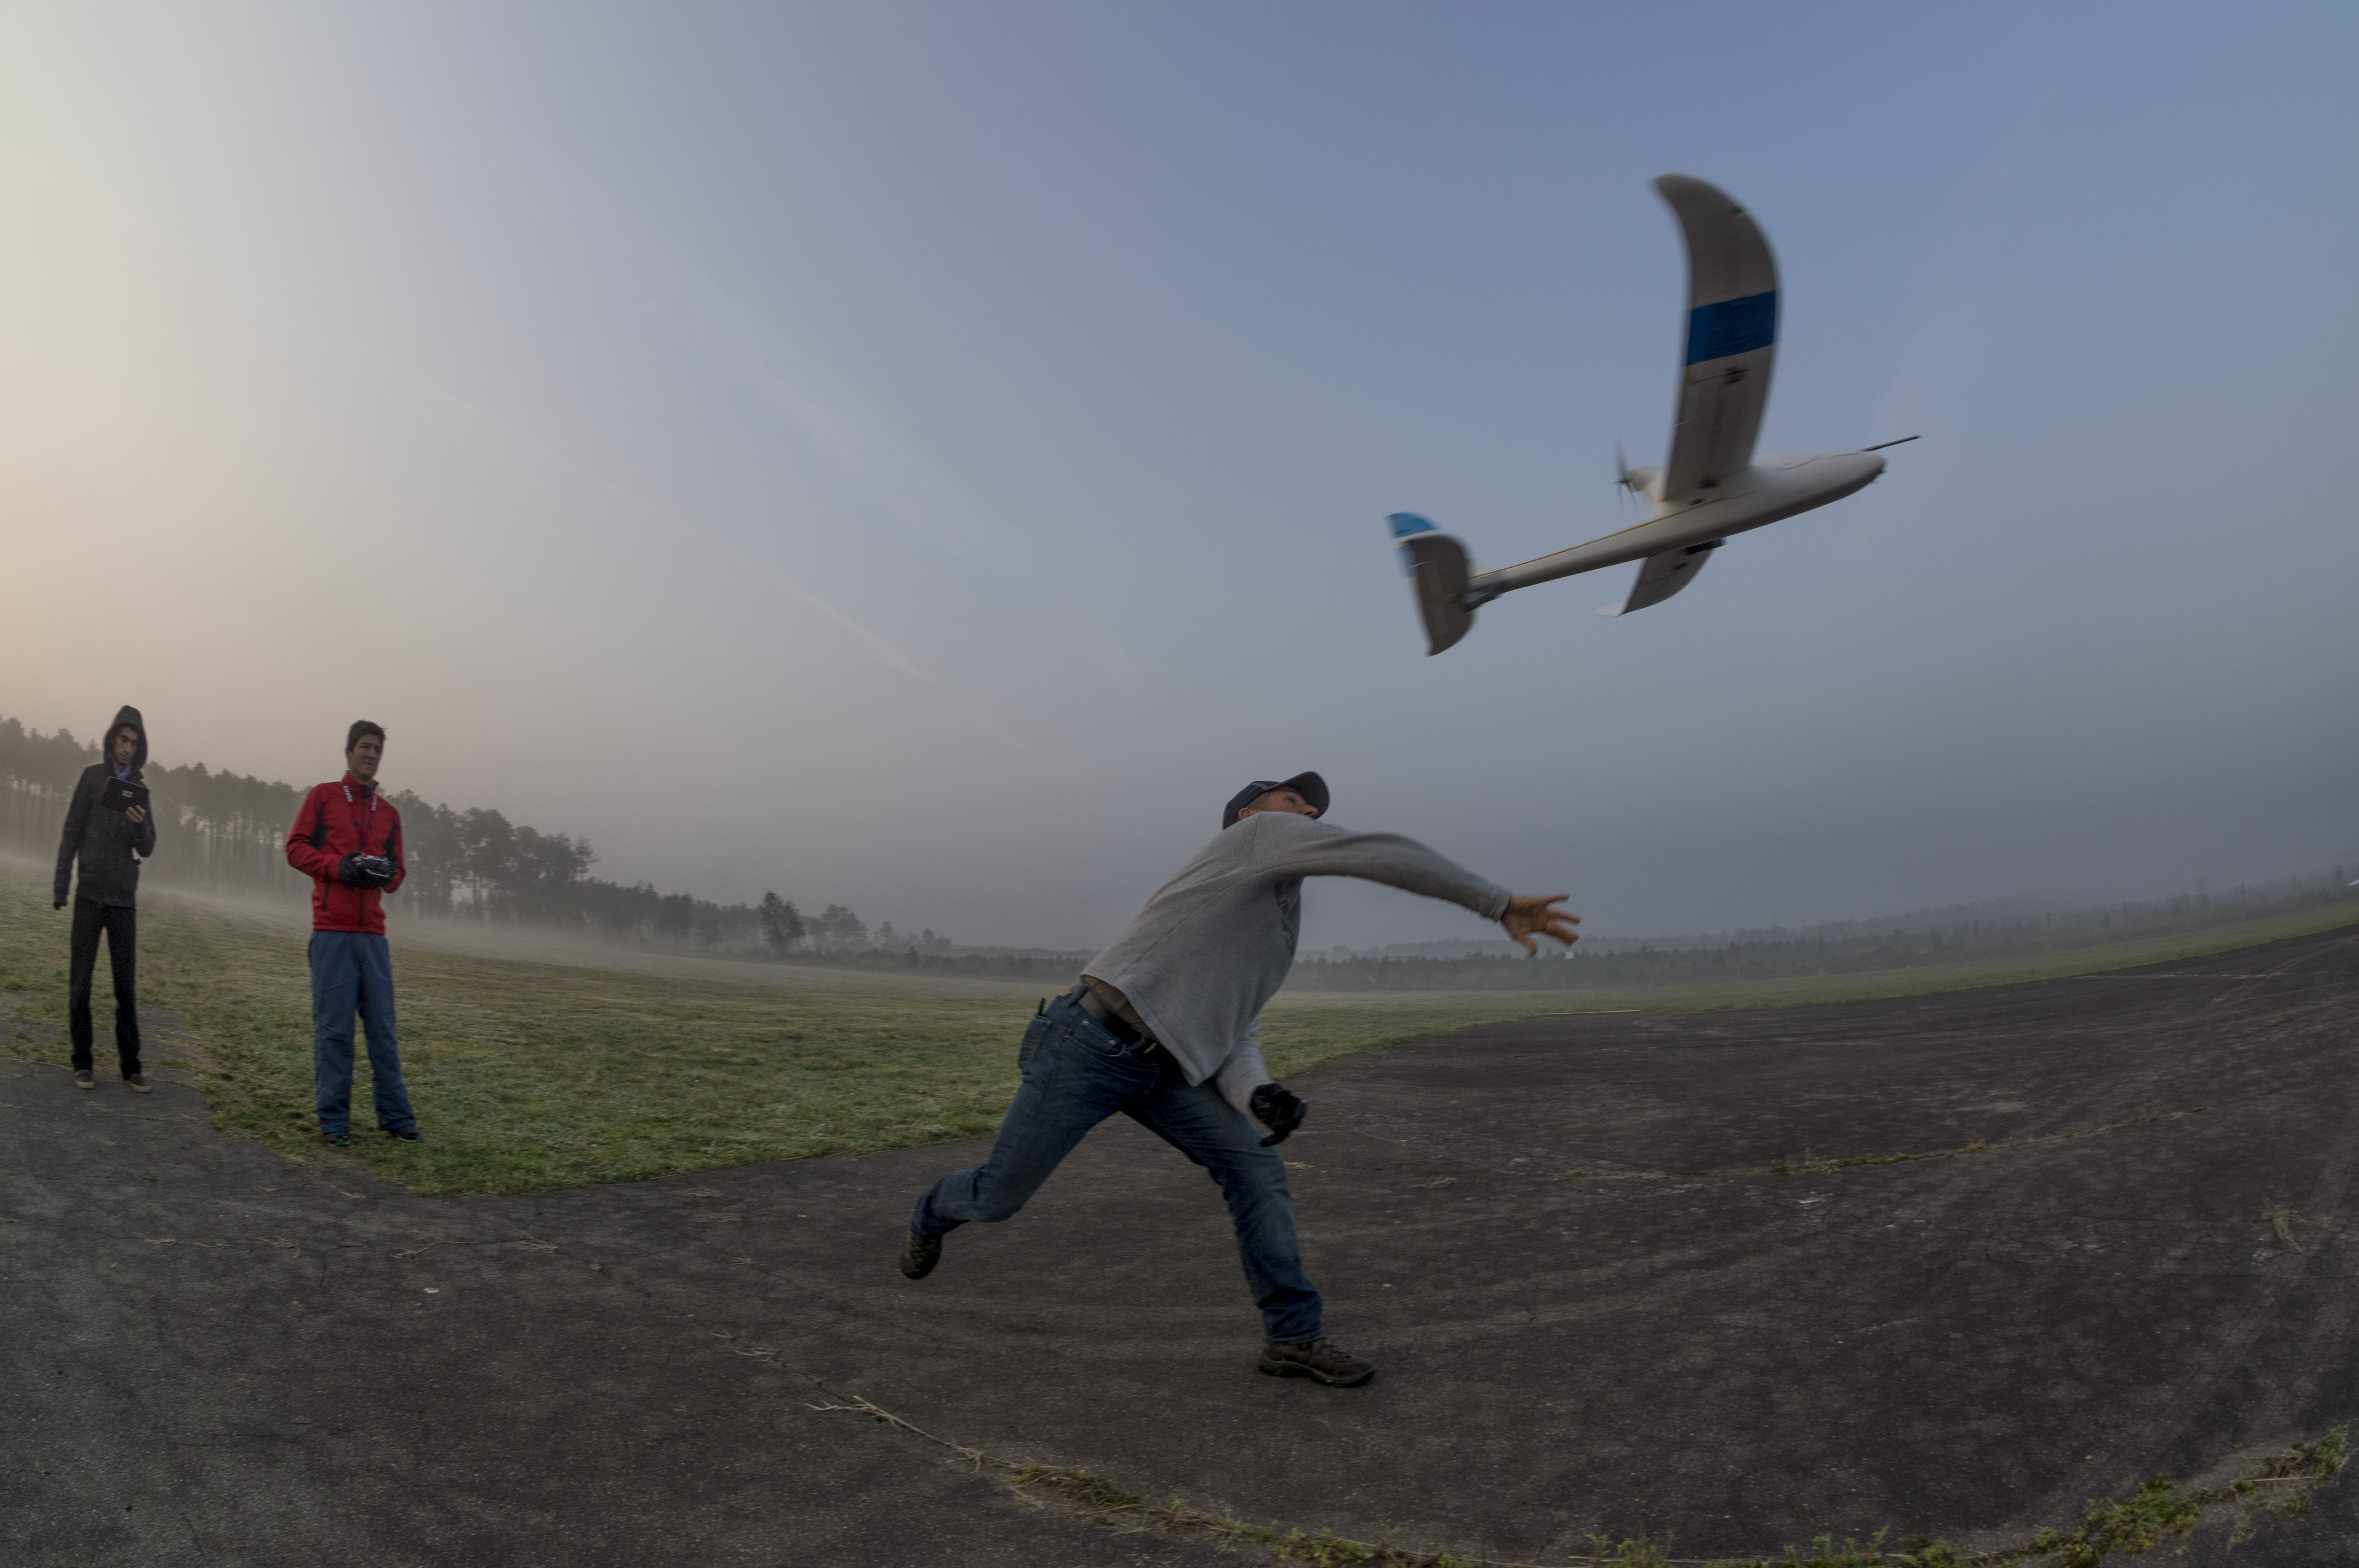
\includegraphics[width=1\textwidth]{figures/flightCampaign}    % The printed column width is 8.4 cm.
\caption{A scene from one of many flight campaigns realized by ENAC UAV laboratory team. Safety pilot can be seen in the photo holding the remote control. Photo taken by Alexandre Bustico.} 
\label{fig:flightCampaign}
\end{center}
\end{figure}

\section{Fault detection from real flight data}

This second section of the chapter discusses the classification results using real flight data. 
Flight campings have been realized in the presence of a safety pilot to recover the drone in case of loss of control when the faults are injected. 
An scene from one of many flight campaigns realized by ENAC UAV laboratory team is given in Fig.~\ref{fig:flightCampaign}. 
Safety pilot can be seen in the photo holding the remote control.

In this section, first, the injection of faults to the flights have been explained throughly. 
The Paparazzi GCS has been altered to inject real-time faults, controllers in some of flight modes have been changed to accommodate faults. 
After, the selection of the faults and nominal phases and also labeling data have been presented. 
Finally, the labeled data have been used to train classifiers for elevon stuck and loss of efficiency faults separately and the classifiers have been evaluated. 
A variety of techniques implemented to improve the performance such as feature engineering and tuning the classifiers. 

\subsection{Injecting faults in flight from Paparazzi GCS}

For the faulty flight data gathering, some modifications to the \emph{Paparazzi} autopilot was necessary in two main parts: Injecting the faults real-time from GCS, and editing the controller onboard so that the sent faulty input values configures the servos as manipulated from the GCS.

\begin{figure}
\begin{center}
\includegraphics[width=22cm,angle=90,origin=c]{figures/groundStationFaultInj}    % The printed column width is 8.4 cm.
\caption{View of fault injection tool in Paparazzi ground control station view of in during flight} 
\label{fig:groundStationFaultInj}
\end{center}
\end{figure}

In order to inject faults real-time from GCS, a slider is added to the GCS to set the fault during flight and set it back to normal flight conditions if necessary.
Fig.~\ref{fig:groundStationFaultInj} shows the GCS view with the fault settings open. 
This pane can be found under  \emph{Settings} $>$  \emph{FAULT} as highlighted in pink in Fig.~\ref{fig:groundStationFaultInj}. 
The four row configuration represents from top to bottom, the multiplicative error in the right elevon, the multiplicative error in the left elevon, additive error in the right elevon, and finally the additive error in the left elevon. 
The nominal condition where there is no fault, is given by $[\begin{matrix}right & left & right\_offset &left\_offset\end{matrix}] = [\begin{matrix} 1.0 & 1.0 & 0 & 0\end{matrix}]$. \\
This configuration lets the user to realize all types of actuator faults, such as control surface inefficiency or stuck. 
To generate the fault of right elevon stuck at its nominal position, setting the first slider ($right$) to zero is enough. 
The generate stuck fault at other positions, $right\_offset$ slider should be changed to desired stuck position while keeping the first slider at zero.
As soon as \emph{Settings} is changed from the GCS (from nominal to faulty or from faulty to nominal), a message is saved to \emph{Paparazzi Messages} (onboard SD card) with the values set in the GCS as shown in Fig.~\ref{fig:flightDataSettings} (SETTINGS Message). 
This message includes the time (the moment that the \emph{Settings} have been changed from the GCS), the aircraft number, and the values set from the GCS ($[\begin{matrix}right & left & right\_offset &left\_offset\end{matrix}]$).

\begin{figure}[h]
\begin{center}
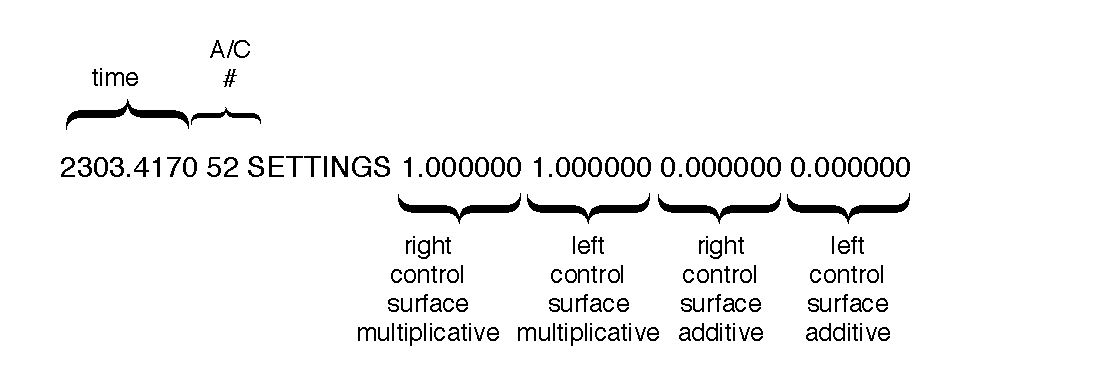
\includegraphics[width=13cm]{figures/flightDataSettings}    % The printed column width is 8.4 cm.
\caption{\emph{SETTINGS} \emph{Message} saves the multiplicative and additive fault values inserted from the GCS.  [1.0 1.0 0.0 0.0] corresponds a command from the GCS to revert back to nominal phase} 
\label{fig:flightDataSettings}
\end{center}
\end{figure}

\subsection{Modifications to \emph{Paparazzi} autopilot controls to inject faults during flight}

For the second part, which is to modify the servo command from the autopilot to the servos, a look at the \emph{Paparazzi} flight modes is necessary. 
Most of the times, there are three modes for fixed-wings from control perspective:  \emph{Auto 1},  \emph{Auto 2},  \emph{Manual}. 
In  \emph{Auto 1}, the pilot is still in the loop and gives the desired pitch and roll values to the controller and the desired elevator and aileron commands are calculated by the autopilot and passed to control allocation where the final desired servo commands are sent to servos as highlighted  \emph{Auto 1} in Fig.~\ref{fig:paparazziControlModes}. 
In the  \emph{Auto 2} mode, there is no need for the pilot since the navigation is also held by the autopilot for a given flight plan. 
This mode is also given as  \emph{Auto 2} in Fig.~\ref{fig:paparazziControlModes}.
In  \emph{Manual} mode, the pilot gives the desired elevator and aileron commands and desired servo commands are calculated in the autopilot's control allocation phase. So still there is a very low sense of autonomy in the manual phase. 

\begin{figure}[h]
\begin{center}
%\includegraphics[width=17cm]{figures/paparazziControlModes}    % The printed column width is 8.4 cm.
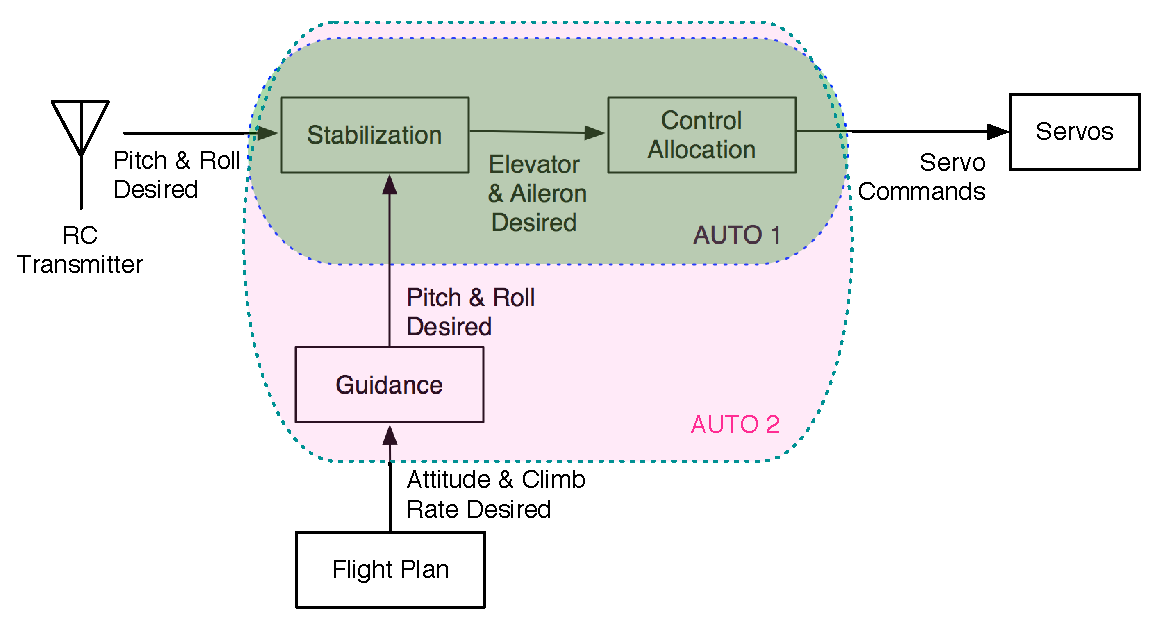
\includegraphics[width=0.9\textwidth]{figures/pprzControlModes}    % The printed column width is 8.4 cm.
\caption{Paparazzi autonomy modes} 
\label{fig:paparazziControlModes}
\end{center}
\end{figure}

Flying with faults is a challenge. 
The risk to crash is increased on purpose, so a back up plan is necessary to recover from faulty situations if the drone seems to be out of control and/or about to crash. 
For that purpose, the faults are only injected to \emph{Auto} modes and \emph{Manual} mode is always free of faults even a fault is given from the ground station. 
So, when the pilot sees a safety problem during the faulty operation, s/he can switch to \emph{Manual} mode from the remote controller and have the control of the control surfaces free from faults. 
Depending on the nature of the fault injected, such as for some severe stuck control surface fault data gatherings, this might be a game changer since the drone would crash unless an action taken.  
This is shown in Fig. ~\ref{fig:faultInjectionPaparazzi} with a switch initiated by the pilot's remote control. 

\begin{figure}[h]
\begin{center}
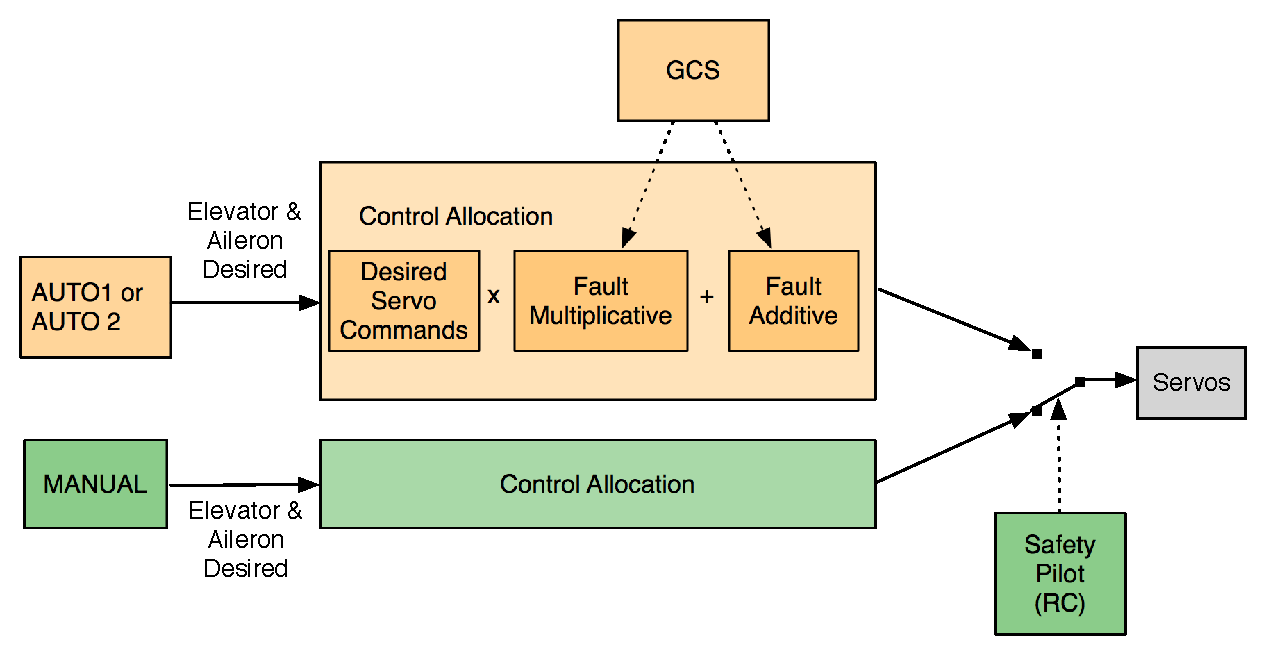
\includegraphics[width=0.9\textwidth]{figures/faultInjectionPprz}    % The printed column width is 8.4 cm.
%\includegraphics[width=19cm,angle=90,origin=c]{figures/faultInjectionPaparazzi}    % The printed column width is 8.4 cm.
\caption{Modifications on the control modes of \emph{Paparazzi} autopilot} 
\label{fig:faultInjectionPaparazzi}
\end{center}
\end{figure}

This figure shows that during the control allocation phase, which is the calculation of the desired servo commands from given desired elevator/aileron commands, faults are injected if the mode is \emph{Auto 1} and \emph{Auto 2} when fault multiplicative or fault additive values are changed from the GCS by the operator.  When switched to \emph{Manual} mode, the control allocation do not consider the injected faults. 

The modifications in the control allocation code to consider additive and multiplicative faults can be seen in the \emph{Paparazzi} code (in C) given below. In \emph{Manual} mode, the servos are not changed by the injected faults. The desired elevator and aileron commands given by the pilot are changed to servo commands by control allocation as usual. In case of \emph{Auto 1} and \emph{Auto 2} modes, control allocation is modified by adding the additive faults ($vfault\_offset\_left$,$vfault\_offset\_right$) and multiplying by multiplicative faults ($vfault\_left$,\ $vfault\_right$). This changes the calculation of servo commands ($AILEVON\_{LEFT}$ and $AILEVON\_{RIGHT}$) in the line of code ($set \ servo = AILEVON\_{LEFT}$ and $set \ servo = AILEVON\_{RIGHT}$). In case of a nominal flight or setting the drone back into the nominal flight, since the multiplicative faults ($vfault\_left$,\ $vfault\_right$) are set to 1.0 and additive faults ($vfault\_offset\_left$,$vfault\_offset\_right$) are set to 0.0, the allocation of the control commands into the servo commands are not modified. In case of \emph{Manual} mode, the autopilot ignores the fault injection with the same idea (multiplicative faults ($vfault\_left$,\ $vfault\_right$) are set to 1.0 and additive faults ($vfault\_offset\_left$, \\ $vfault\_offset\_right$) are set to 0.0)


\lstset{language=C}
\begin{lstlisting}

  <command_laws>
    <let var="aileron" value="@ROLL  * AILEVON_AILERON_RATE"/>
    <let var="elevator" value="@PITCH * AILEVON_ELEVATOR_RATE"/>
    <let var="manual" value="(fbw_mode==FBW_MODE_MANUAL)"/>
    <let var="vfault_left" value="100 * ($manual ? 1 : fault_left)"/>
    <let var="vfault_right" value="100 * ($manual ? 1 : fault_right)"/>
    <let var="vfault_offset_left" value="($manual ? 0 : fault_offset_left)"/>
    <let var="vfault_offset_right" value="($manual ? 0 : fault_offset_right)"/>
    <set servo="MOTOR" value="@THROTTLE"/>
    <set servo="AILEVON_LEFT" value="(($elevator - $aileron) * $vfault_left) / 100 + $vfault_offset_left"/>
    <set servo="AILEVON_RIGHT" value="(($elevator + $aileron) * $vfault_right) / 100 + $vfault_offset_right"/>
  </command_laws>
  
\end{lstlisting}


\subsection{Reading \& labeling flight data}


Flight data saved to the SD card onboard should be converted to \emph{data} format by using the \textit{sd2log} program of \emph{Paparazzi}. For that purpose, from the terminal, browse into the folder including the log file in \emph{LOG} format, which is the file format for the onboard data saved in Paparazzi. 

\begin{figure}[h]
\begin{center}

\includegraphics[width=15cm]{figures/dataManip}    % The printed column width is 8.4 cm.
\caption{Conversion of raw flight data saved to SD card onboard to .data file to be used in further calculations} 
\label{fig:dataManip}
\end{center}
\end{figure}

Run the program under paparazzi/sw/logalize/sd2log and specify the file is to be converted to \emph{.data} format and where to export it as shown in Fig.~\ref{fig:dataManip} ('.' means extract to current folder). 

An example of a part of the flight data\footnote{17\_07\_06\_\_10\_21\_07\_SD.data} is given in Fig.~\ref{fig:dataSettingsNominalFault} and whole file is available in \emph{Github}\footnote{https://github.com/benelgiz/cureDDrone/tree/master/ \\ data/v4\_multiplicativeAdditive\_MURET\_06\_07\_2017}. 
The UAV used to realize the faulty flights in order to generate labeled data is given in Fig.~\ref{fig:zagi}. 

\begin{figure}[h]
\begin{center}
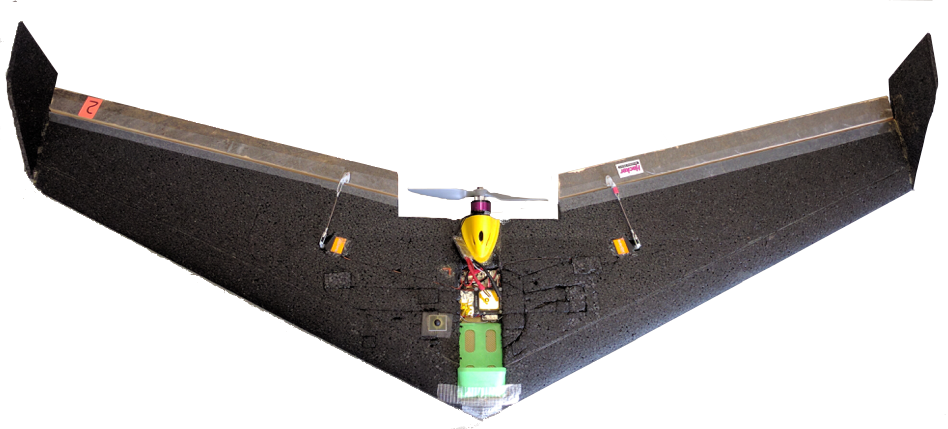
\includegraphics[width=0.87\textwidth]{figures/zagi}    % The printed column width is 8.4 cm.
\caption{The flying-wing: \emph{ZAGI}} 
\label{fig:zagi}
\end{center}
\end{figure}

The duration of the flight was around an hour. 
The flight has been practiced under strong wind. 
34 different faults are injected.
During the flight, the effect of the faults on the drone was sometimes visible to human eye and sometimes not. 
For the control surface stuck faults, even for one control surface was stuck case, it immediately gets out of control and safety pilot takes the initiative. 
Thanks to the piloting skills, no crashes occurred. 
For ineffectiveness of control surface faults, where the controller has still an effect but not as efficient as before, error in navigation was observed.  

\begin{figure}
\begin{center}
\includegraphics[width=10.1cm]{figures/dataSettingsNominalFault}    % The printed column width is 8.4 cm.
\caption{A piece of the flight data corresponding to nominal and two different fault phases of the flight. \emph{SETTINGS} message exists only if there is a change in the multiplicative and additive fault parameters via GCS. The first data in each row corresponds to the time stamp. Second data in each row is the aircraft number which is 52 for this flight. Third data in each data line corresponds to the label of information in that line. As an example, on the last line, the label is $IMU\_ACCEL$. This means that this line gives accelerometer readings. Last three data in this line are accelerometer x-axis (-1.187500), accelerometer y-axis (-0.916992) and accelerometer z-axis (-1.717773) readings.} 
\label{fig:dataSettingsNominalFault}
\end{center}
\end{figure}


After converting the flight data file to \emph{.data} format, the file can be read from Matlab. Next step is to detect the time stamps at which the faults are injected and then label all the data corresponding to this fault interval as designated with different colors in Fig.~\ref{fig:dataSettingsNominalFault}. 
Since, most of the times, there has been more than one fault type generated during flights, another step in data manipulation is to choose the faults to investigate. 

The fault injection or change from fault condition to nominal mode is done via the GCS and there is a corresponding message saved to SD card onboard in \emph{Paparazzi} \emph{Messages} indicated via \emph{Settings}. 
\emph{Settings} gives multiplicative fault and additive fault values and only appears in the flight data when one of the control surface effectiveness values is changed. 
The value of the \emph{Settings} for nominal phase is [1.0 1.0 0.0 0.0] and a corresponding example line in the data corresponding to a command to revert to nominal condition can be seen in Fig.~\ref{fig:flightDataSettings}. 

It means to multiply the value given by the controller by 1 and add 0, so does not change the values given by the autopilot. 
As soon as any of control surface effectiveness values is changed in the GCS, a new \emph{Settings} value is saved to the file (Shown with arrows in Fig.~\ref{fig:dataSettingsNominalFault}). 

To find the indexes where the nominal and faulty data starts and ends, the values of the  \emph{Settings} message is investigated. 
So when there is a  \emph{Settings} message in the flight, it should be either a fault generation or going back to nominal condition after a fault. 
If the message contains the  \emph{Settings} message equal to [1.0 1.0 0.0 0.0], this data index is selected as the nominal condition start index and a previous index before next  \emph{Settings} message is the last index of this nominal phase. 
The matrix holding the start and end index for the nominal phases are saved as \textit{nominal\_start\_stop} shown in Table~\ref{arm:tableNominalindexes} where the first row corresponds to start index of each nominal set and second row corresponds to the last index of the corresponding as nominal phase. 

\newcolumntype{M}[1]{>{\centering\arraybackslash}m{#1}}

\begin{table}
\caption{Nominal phase start stop indexes of the flight}
\label{arm:tableNominalindexes}
\begin{center}
\begin{tabular}{ ||m{4.7cm}|m{1.3cm}|m{1.3cm}|m{1.3cm}|m{1.3cm}|m{1.3cm}|m{1.3cm}|m{1.3cm}|m{1.3cm}|m{1.3cm}|m{1.3cm}|m{1.3cm}||}\hline
\textbf{nominal phase number} & 2 & 3 & 4 & 5 & $\cdots$ & 12 \\\hline
\vtop{\hbox{\strut \textbf{nominal start }}\hbox{\strut \textbf{nominal\_start\_stop(1,:)}}} & 516919 & 551627 & 755227	& 824545	& $\cdots$ & 1048055 \\\hline
\vtop{\hbox{\strut \textbf{nominal stop}}\hbox{\strut \textbf{nominal\_start\_stop(2,:)}}} & 521965 & 622015 & 782580 & 924704 & $\cdots$ & 1065548 \\\hline
\end{tabular}
\end{center}
\end{table}

For the fault indexes a similar approach is followed except that  \emph{Settings} messages selected are the ones which is different than  [1.0 1.0 0.0 0.0]. 
An example is Fault \#23 in Fig.~\ref{fig:settingsStuckFault} and its corresponding start and end indexes given in Table~\ref{arm:tableFaultyindexes}.

\begin{figure}[h]
\begin{center}

\includegraphics[width=11cm]{figures/settingsStuckFault}    % The printed column width is 8.4 cm.
\caption{SETTINGS message corresponding to stuck of right control surface} 
\label{fig:settingsStuckFault}
\end{center}
\end{figure}

\newcolumntype{M}[1]{>{\centering\arraybackslash}m{#1}}

\begin{table}[h]
\caption{Faulty phase start stop indexes of the flight}
\label{arm:tableFaultyindexes}
\begin{center}
\begin{tabular}{ ||m{4.7cm}|m{1.3cm}|m{1.3cm}|m{1.3cm}|m{1.3cm}|m{1.3cm}|m{1.3cm}|m{1.3cm}|m{1.3cm}|m{1.3cm}|m{1.3cm}|m{1.3cm}||}\hline
\textbf{fault phase number} & 1 & 2 &  $\cdots$ & 23 & $\cdots$ & 34 \\\hline
\vtop{\hbox{\strut \textbf{fault start }}\hbox{\strut \textbf{fault\_start\_stop(1,:)}}} & 456888 & 473827 & $\cdots$	& 924705	& $\cdots$ & 1076847 \\\hline
\vtop{\hbox{\strut \textbf{fault stop}}\hbox{\strut \textbf{fault\_start\_stop(2,:)}}} & 473826 & 485762 & $\cdots$ & 925390 & $\cdots$ & 1077117 \\\hline
\end{tabular}
\end{center}
\end{table}


Next step is to choose the phases of the flight to work with. 
As an example, a phase of the flight where there is enough nominal data and followed with an extreme fault injection is selected. 
This corresponds to the 4th nominal phase of the flight followed by the 23th fault is selected. Fault \#23 corresponds to right control surface stuck and can be seen in  Fig.~\ref{fig:dataSettingsNominalFault}. 
The next is to select the measurement corresponding the these selected time intervals and this is done by AND ing the indexes of interest, such as the indexes of fault and gyro data measurements as shown in Fig.~\ref{fig:labelingGyroAccel}. 
The script for labeling the nominal and faulty measurements is the \emph{selectDataToInvest.m} file given in Appendix B.2. 
The output of this file is the accelerometer and gyro measurements corresponding to selected phases of the flight.

\begin{figure}[h]
\begin{center}
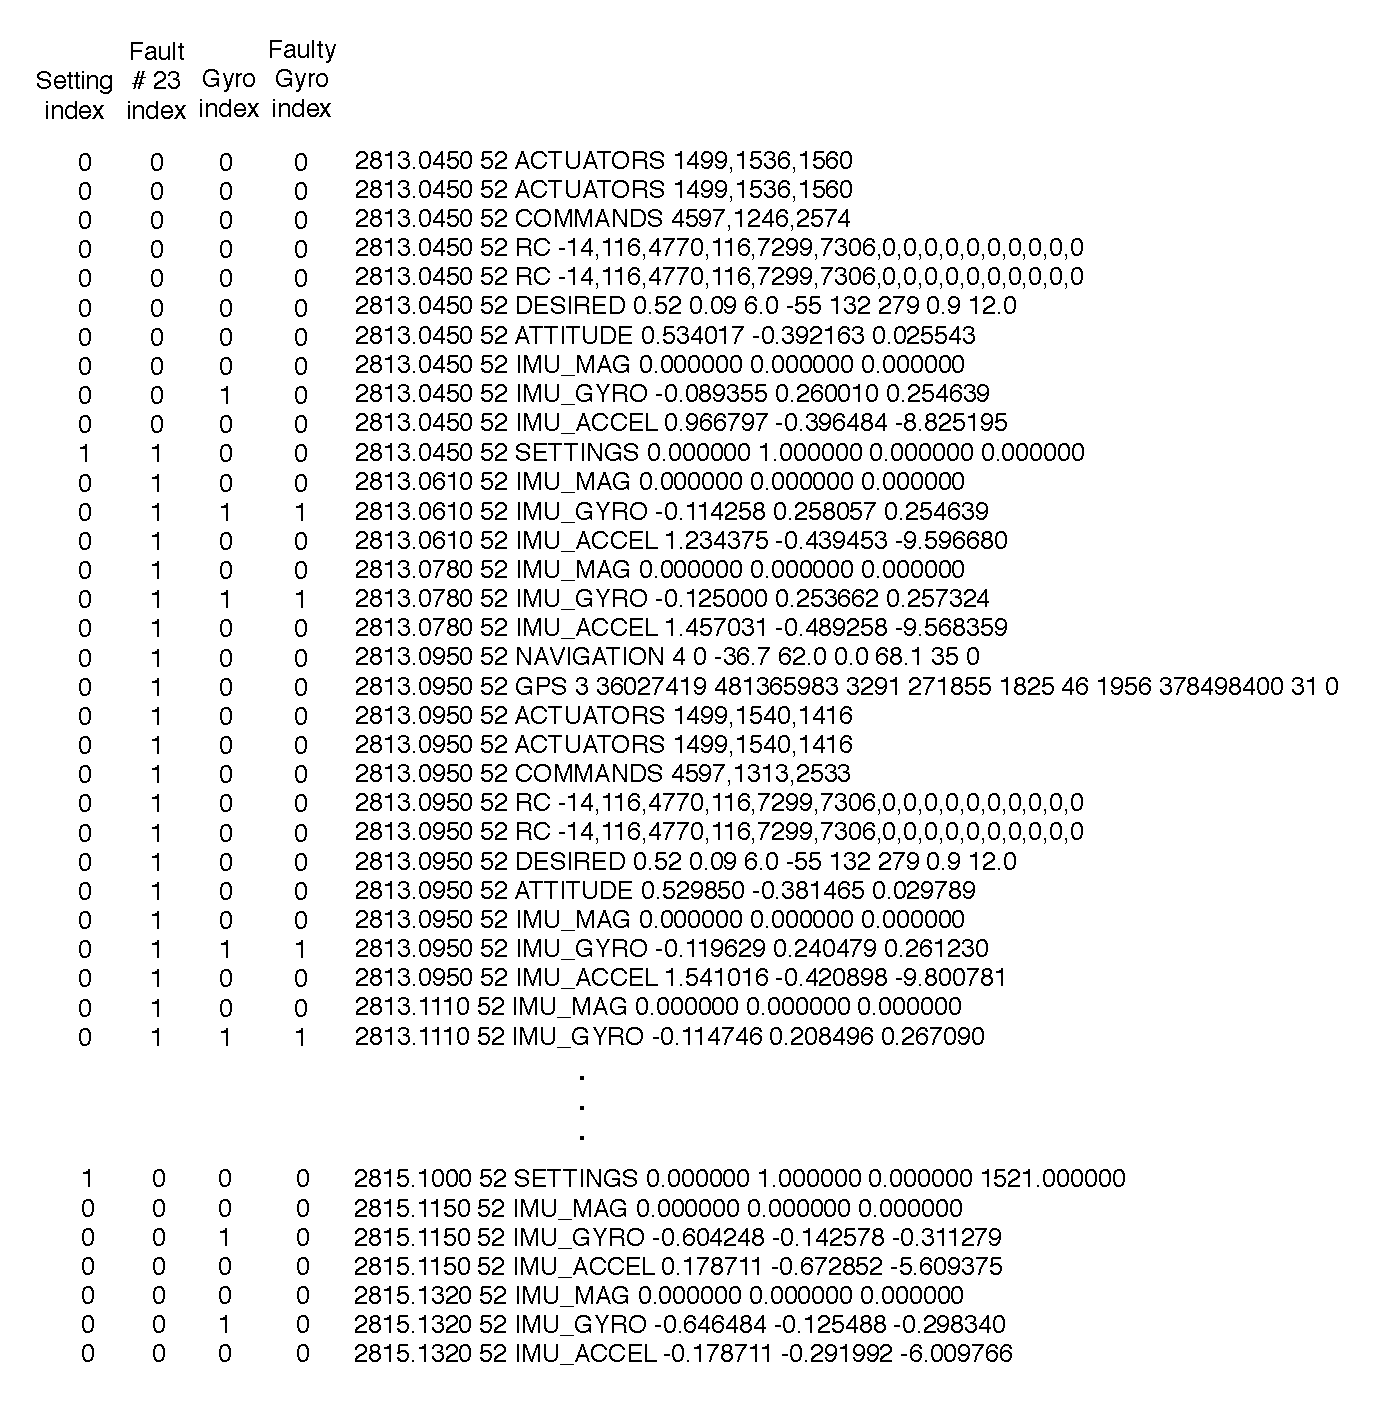
\includegraphics[width=15.1cm]{figures/labelingGyroAccel}    % The printed column width is 8.4 cm.
\caption{Indexing SETTINGS, to find fault and nominal flight intervals, indexing GYRO measurements to AND with FAULT indexes to find the indexes of faulty gyro measurements} 
\label{fig:labelingGyroAccel}
\end{center}
\end{figure}

SVM classifier has been trained and tuned with the flight data, generated by following the steps covered above, in order to classify the faulty and nominal classes.
The simulations have been developed under Matlab coding environment. 
Some tools, such as calculation of \emph{f1Score}, were written as Matlab scripts rather than changing some arguments of toolbox functions, since they were not found available in the toolbox either it does not exist or was difficult to obtain.
 
The simulations have been executed on HP Z820 Workstation with 3.1 GHz, 32 cores. 
 
This work investigates only binary classification, not multi-class classification considering multiple different faults.  
But different faulty cases have been studied to further attack the problem of multi-class classification in the future studies. 
The classifier's abilities in different fault conditions have been investigated. 
The main two types of faults of interest in this study were control surface stuck and LOE. 
The flight data\footnote{https://github.com/benelgiz/cureDDrone/tree/master/ \\ data/v4\_multiplicativeAdditive\_MURET\_06\_07\_2017} and code\footnote{https://github.com/benelgiz/cureDDrone/tree/master} that has been developed are publicly available under \emph{Github}.

All three steps (training, tuning and evaluation), explained thoroughly under SVM application section have been applied and the results are given below.

\subsection{Control surface stuck fault}

During the flights, the most challenging fault to realize was the control surface stuck. 
The drone reacted very fast with an uncontrollable dive towards the ground and the safety pilot initiated manual recovery by triggering the safety switch shown in Fig.~\ref{fig:faultInjectionPaparazzi}. 
So the time past starting from the ignition of the control surface stuck fault until the manual pilot's intervention is very short ($\sim$2 seconds) which can be seen from the accelerometer x-direction readings in Fig.~\ref{fig:acc_x}. 

This causes the problem of skew-class classification where there is a big difference between the number of instances belonging to different classes and requires some special treatment as explained above under section ~\ref{evalClassifier}.

\begin{figure}[H]
\begin{center}
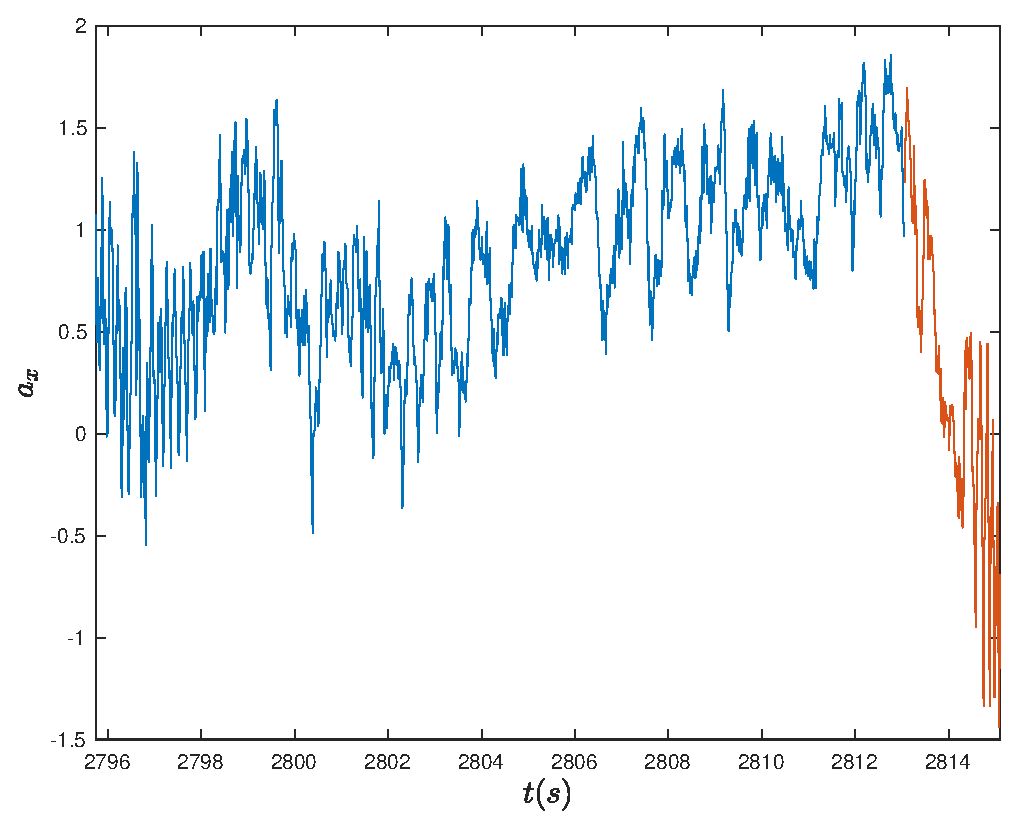
\includegraphics[width=0.7\textwidth]{figures/acc_x}    % The printed column width is 8.4 cm.
\caption{Accelerometer readings along $x$-direction during flight interval just before control surface stuck (nominal, represented with blue) and during control surface stuck at $\SI{0}{\degree}$ until the safety pilot's intervention} 
\label{fig:acc_x}
\end{center}
\end{figure}

First problem considered for classification is the right elevon stuck at $\SI{0}{\degree}$.
Gyro and accelerometer measurements are saved to SD card onboard at 60 Hz. 
Nominal class involves $\sim$5 minutes of accelerometer and gyro data while the faulty class comprised of $\sim$2 seconds of data, thus the problem is treated as skew-class classification. 

Having knowledge about data is critical for machine learning applications. 
Usually, the performance of the learning algorithms are quite dependent on the level of the engineer's experience since some of the critical decision are handled by her/him such as selection of features (not for all machine learning methods).
Fig.~\ref{fig:acc_x} shows accelerometer x-axis measurements for a duration of $\sim$20 seconds. 
Measurements plotted in blue indicates the part of the flight where elevon works correctly while red part of the plot corresponds to the faulty phase. 
It can be interpreted from the Fig.~\ref{fig:acc_x} that the fault injected shows a distinct change in the x-axis accelerometer measurements when the fault is injected. 

\begin{figure}[H]
\begin{center}
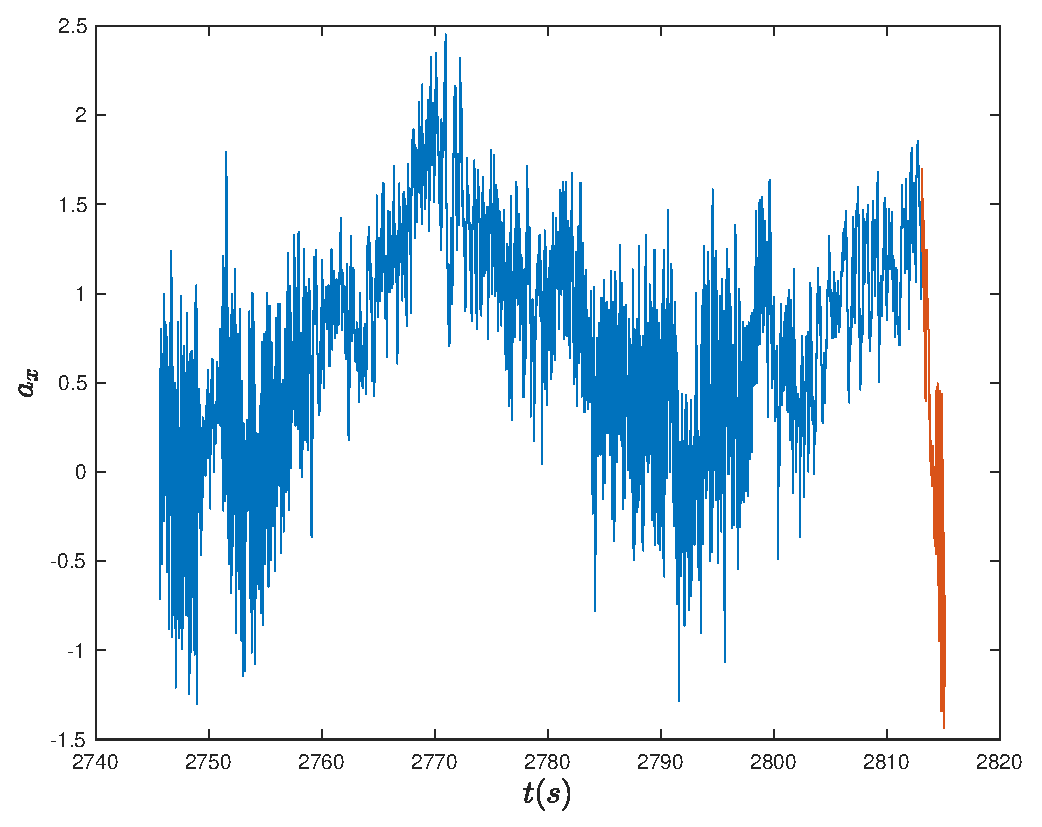
\includegraphics[width=0.78\textwidth]{figures/acc_x_evenLongerNominal}    % The printed column width is 8.4 cm.
\caption{Accelerometer readings along $x$-direction during flight interval before control surface stuck (nominal, represented with blue) and during control surface stuck at  $\SI{0}{\degree}$ until the safety pilot's intervention} 
\label{fig:acc_x_evenLongerNominal}
\end{center}
\end{figure}



%\begin{figure}
%\begin{center}
%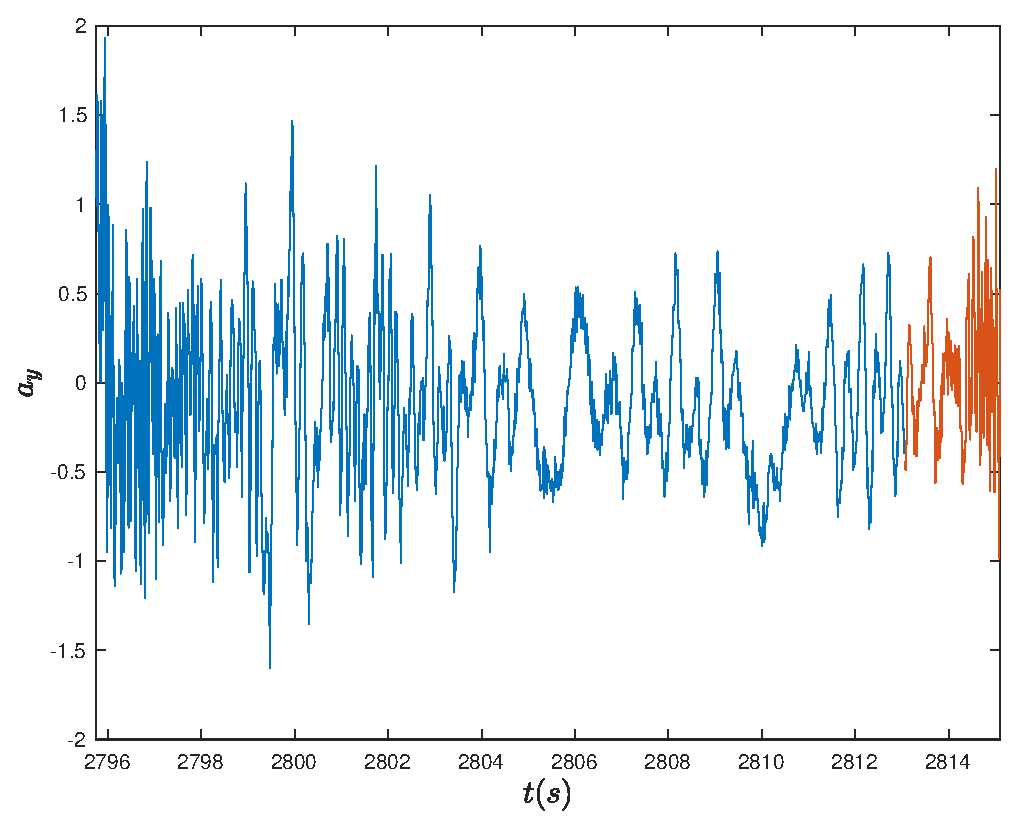
\includegraphics[width=11cm]{figures/acc_y}    % The printed column width is 8.4 cm.
%\caption{$a_x$ vs $a_y$ feature space for faulty nominal flight data} 
%\label{fig:acc_y}
%\end{center}
%\end{figure}

%\begin{figure}
%\begin{center}
%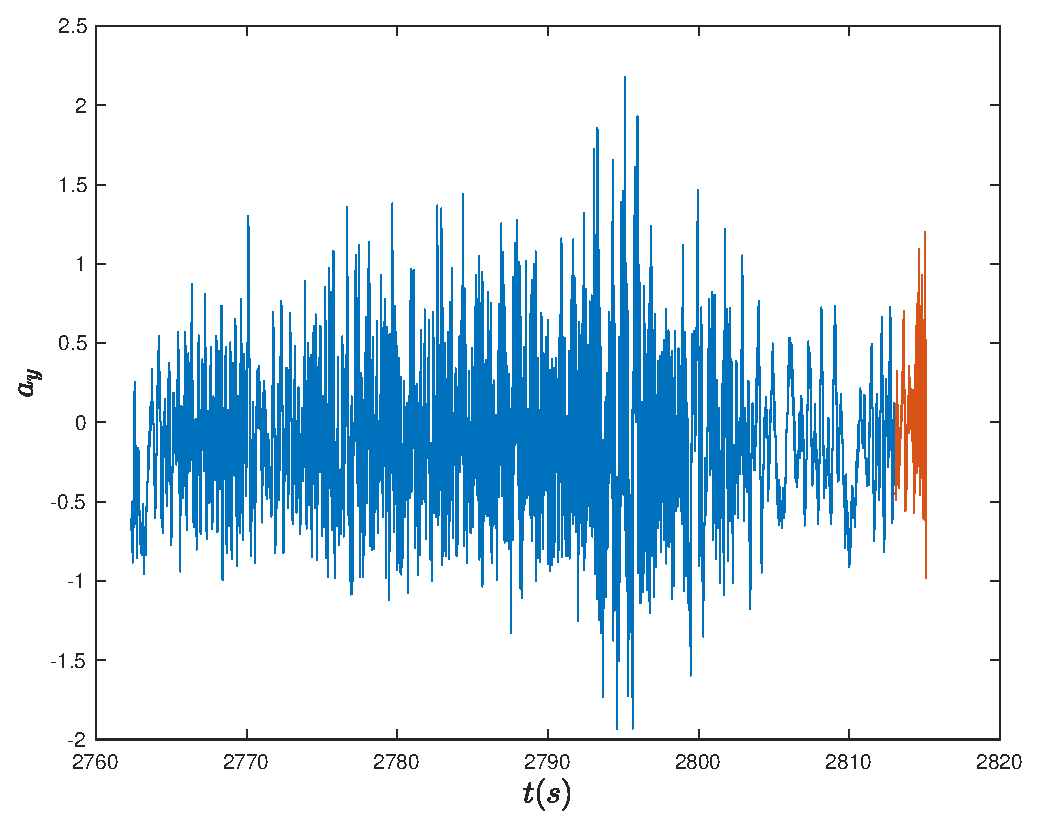
\includegraphics[width=11cm]{figures/acc_y_longNominal}    % The printed column width is 8.4 cm.
%\caption{$a_x$ vs $a_y$ feature space for faulty nominal flight data} 
%\label{fig:acc_y_longNominal}
%\end{center}
%\end{figure}



To investigate further, measurements have been plotted during a larger time scale involving $\sim$70 seconds of measurements as shown in Fig.~\ref{fig:acc_x_evenLongerNominal}. 
Here, it is seen that the accelerometer measurements corresponding to faulty phase could be observed during the nominal flight phase as well, thus it might be necessary to check the time change of translational acceleration to catch a difference in behavior. 

Fig.~\ref{fig:acc_z} and Fig.~\ref{fig:gyro_x} show the accelerometer measurements along z-direction and angular velocities along x-direction during a short time interval. 
Here, although an average of faulty measurements would result in an obvious difference, individual measures might correspond to nominal phase of the flight as well.

The measurements are also plotted in feature spaces $a_x$-$a_z$ and $a_x$-$a_y$ as shown in Fig.~\ref{fig:feat1vsfeat3FaultStuck} and Fig.~\ref{fig:feat1vsfeat2FaultStuck}. 
It shows $a_x$-$a_z$ space gives a distribution that would be easier to classify the faulty and nominal phases while in $a_x$-$a_y$ feature space, the measures are quite similar and difficult to classify.


\begin{figure}[H]
\begin{center}
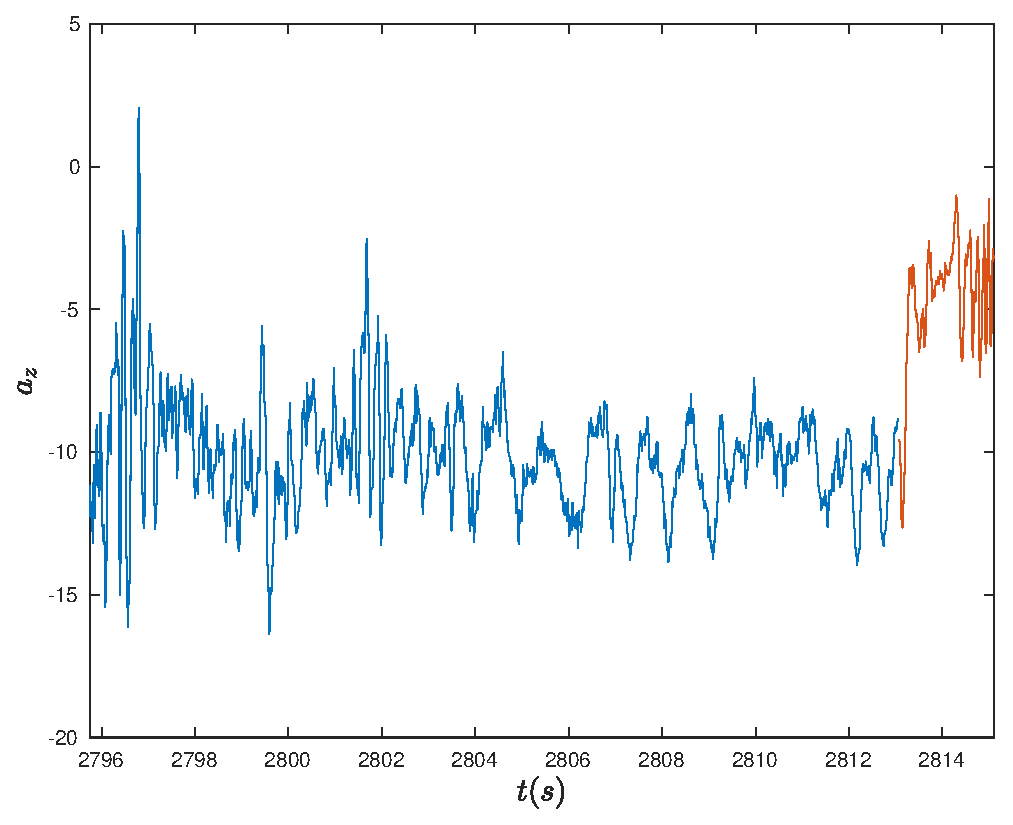
\includegraphics[width=0.66\textwidth]{figures/acc_z}    % The printed column width is 8.4 cm.
\caption{Accelerometer measurements along z direction $a_z$ for faulty and nominal flight data} 
\label{fig:acc_z}
\end{center}
\end{figure}

\begin{figure}[H]
\begin{center}
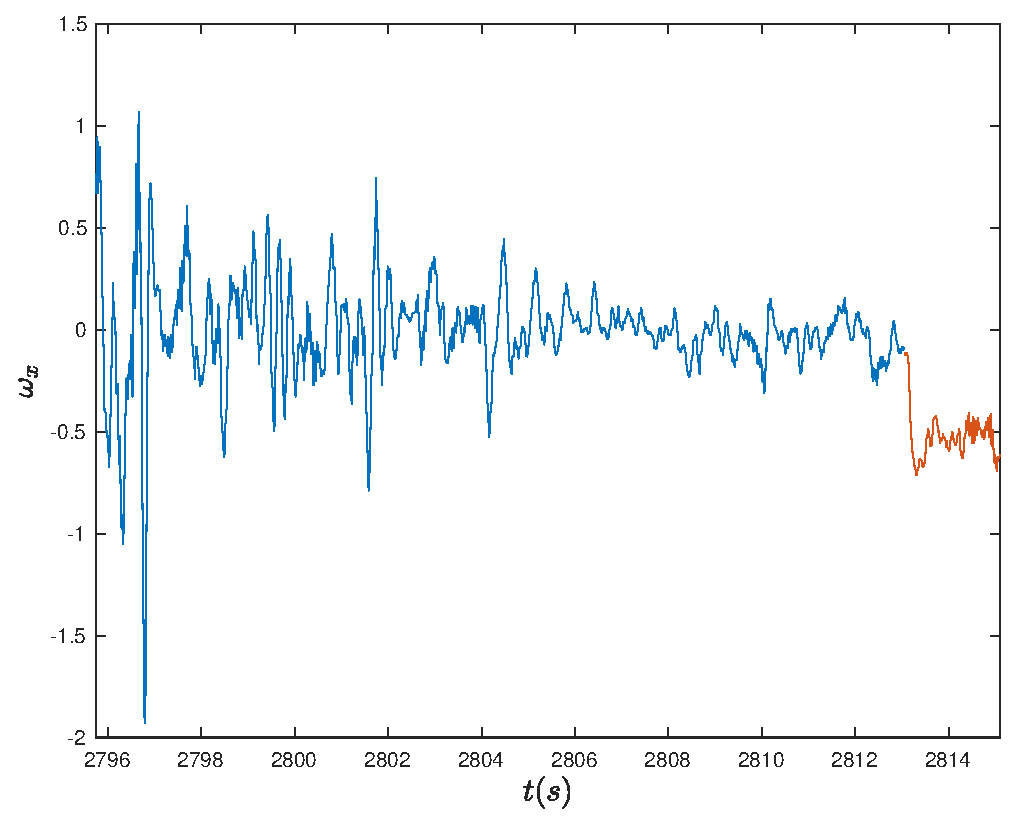
\includegraphics[width=0.65\textwidth]{figures/gyro_x}    % The printed column width is 8.4 cm.
\caption{Angular velocity $w_x$  for faulty nominal flight data} 
\label{fig:gyro_x}
\end{center}
\end{figure}


\begin{figure}[H]
\begin{center}
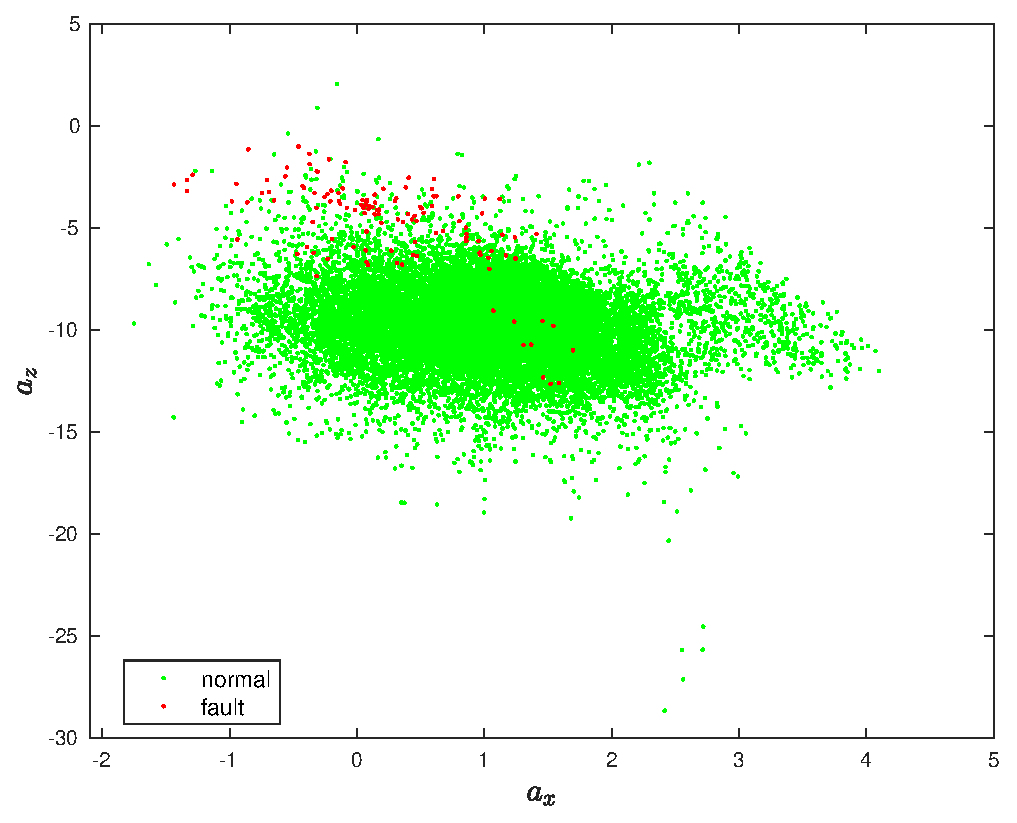
\includegraphics[width=0.65\textwidth]{figures/feat1vsfeat3FaultStuck}    % The printed column width is 8.4 cm.
\caption{$a_x$ vs $a_z$ feature space for faulty nominal flight data} 
\label{fig:feat1vsfeat3FaultStuck}
\end{center}
\end{figure}

\begin{figure}[H]
\begin{center}
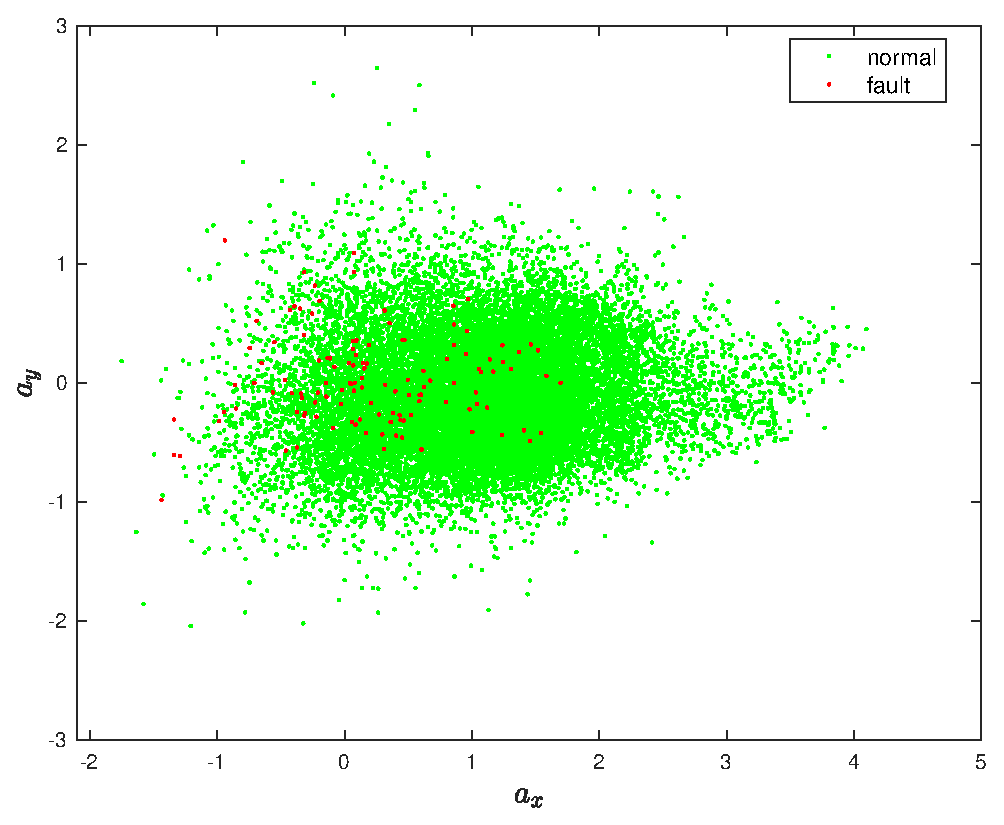
\includegraphics[width=0.65\textwidth]{figures/feat1vsfeat2FaultStuck}    % The printed column width is 8.4 cm.
\caption{$a_x$ vs $a_y$ feature space for faulty nominal flight data} 
\label{fig:feat1vsfeat2FaultStuck}
\end{center}
\end{figure}

%\begin{figure}
%\begin{center}
%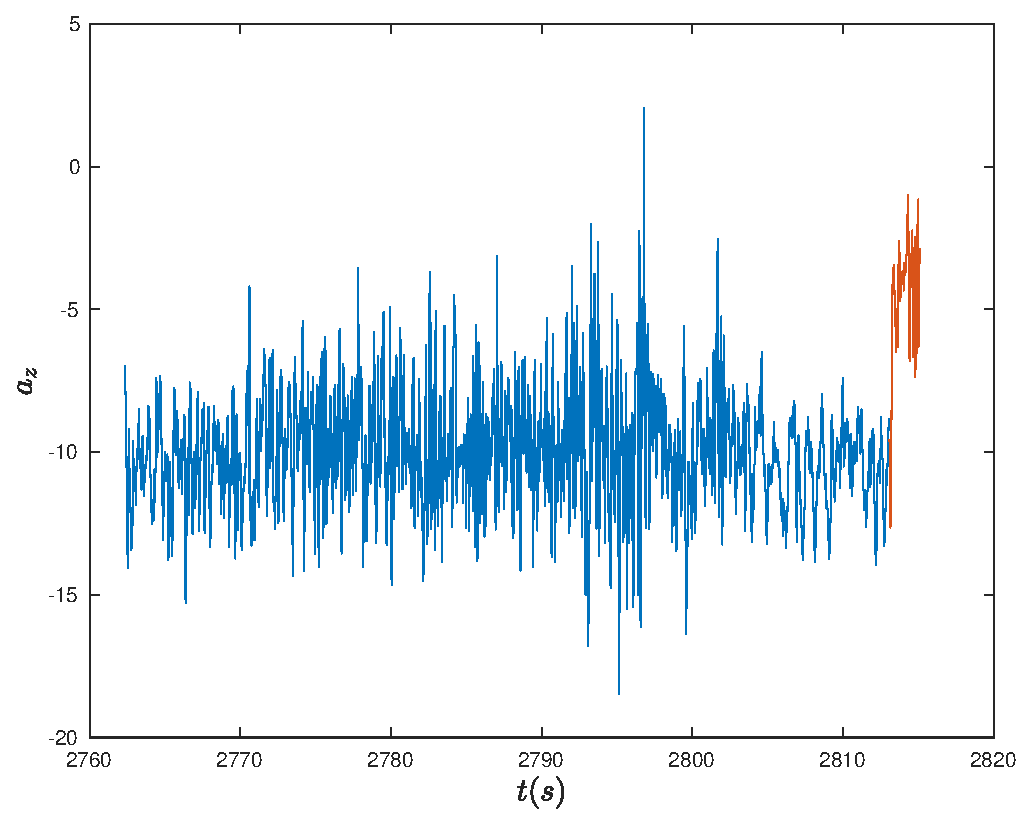
\includegraphics[width=11cm]{figures/acc_z_longNominal}    % The printed column width is 8.4 cm.
%\caption{$a_x$ vs $a_y$ feature space for faulty nominal flight data} 
%\label{fig:acc_z_longNominal}
%\end{center}
%\end{figure}


\begin{table}[!ht]
	\centering
% table caption is above the table
\caption{Untuned and tuned via heuristic approach and tuned via Bayesian optimization SVM classification evaluations}
\label{tab:stuck}       % Give a unique label
% For LaTeX tables use
\begin{tabular}{p{2.7cm}p{2.0cm}p{2.3cm}p{3cm}p{3cm}}
\hline\noalign{\smallskip}
 & Untuned linear kernel & Untuned Gaussian kernel & Tuned heuristic Gaussian kernel & Tuned Bayesian Gaussian kernel\\
\noalign{\smallskip}\hline\noalign{\smallskip}
kernel scale & 1 & 1 & 2.1187 & 10.3581 \\
box constraint & 1 & 1 & 1 & 1323.1 \\
margin & 10.5927 & 2.0248 & 2.4763 & 5.3004 \\
edge & 10.5875 & 2.0245 & 2.4761 & 5.3004 \\
kFoldLoss & 0.2 x $10^{-2}$ & 1.2 x $10^{-3}$& 7.571 x $10^{-4}$ & 1.2 x $10^{-3}$ \\
precision & 0.76 & 1 & 1 & 0.913 \\
recall & 0.8261 & 0.8696 & 0.913 & 0.913\\
\textbf{f1Score} & 0.7917 & 0.9302 &0.9545 & 0.913 \\
comp. time & 3.75s & 3.4s & 5917.5s & 1784.7s \\
\noalign{\smallskip}\hline
\end{tabular}
\end{table}

%\begin{figure}
%\begin{center}
%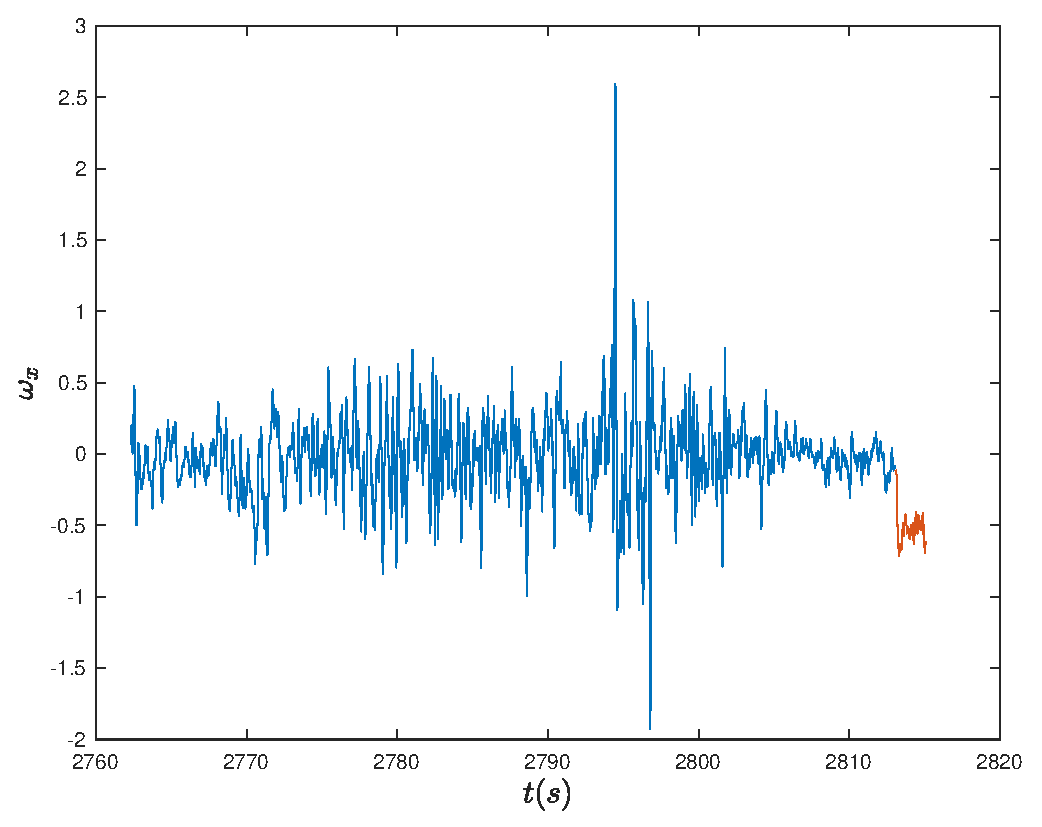
\includegraphics[width=11cm]{figures/gyro_x_longNominal}    % The printed column width is 8.4 cm.
%\caption{$a_x$ vs $a_y$ feature space for faulty nominal flight data} 
%\label{fig:gyro_x_longNominal}
%\end{center}
%\end{figure}

%\begin{figure}
%\begin{center}
%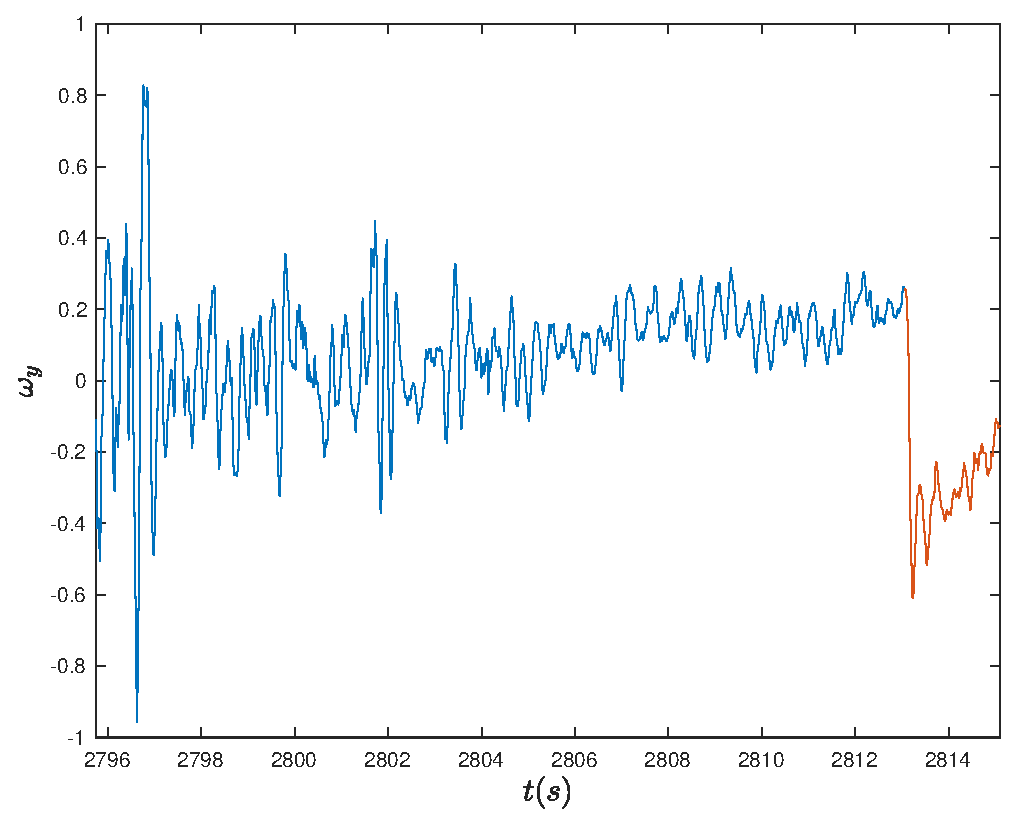
\includegraphics[width=11cm]{figures/gyro_y}    % The printed column width is 8.4 cm.
%\caption{$a_x$ vs $a_y$ feature space for faulty nominal flight data} 
%\label{fig:gyro_y}
%\end{center}
%\end{figure}

%\begin{figure}
%\begin{center}
%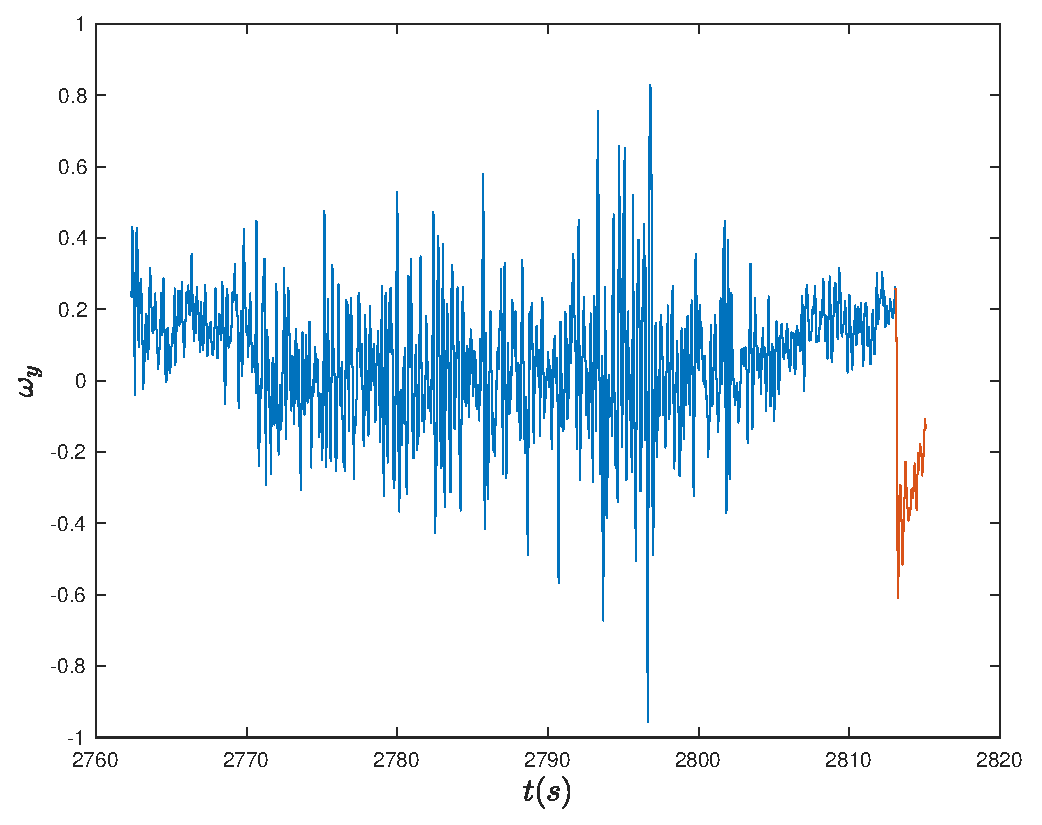
\includegraphics[width=11cm]{figures/gyro_y_longNominal}    % The printed column width is 8.4 cm.
%\caption{$a_x$ vs $a_y$ feature space for faulty nominal flight data} 
%\label{fig:gyro_y_longNominal}
%\end{center}
%\end{figure}

%\begin{figure}
%\begin{center}
%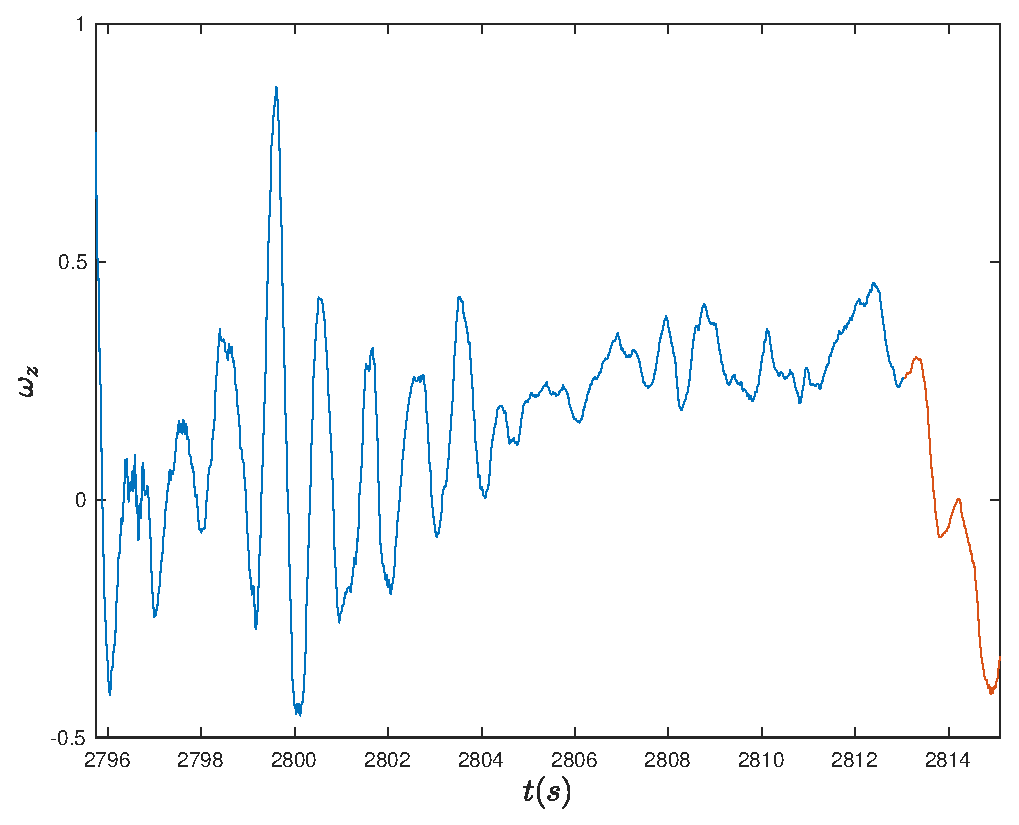
\includegraphics[width=11cm]{figures/gyro_z}    % The printed column width is 8.4 cm.
%\caption{$a_x$ vs $a_y$ feature space for faulty nominal flight data} 
%\label{fig:gyro_z}
%\end{center}
%\end{figure}

%\begin{figure}
%\begin{center}
%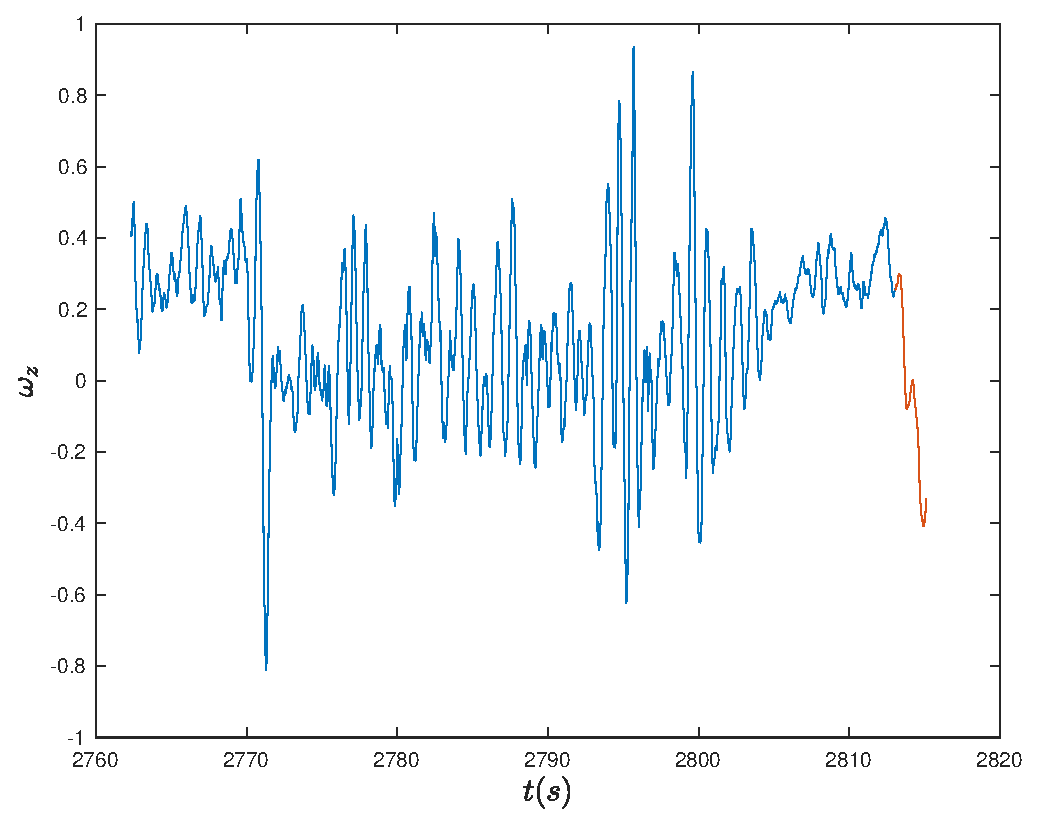
\includegraphics[width=11cm]{figures/gyro_z_longNominal}    % The printed column width is 8.4 cm.
%\caption{$a_x$ vs $a_y$ feature space for faulty nominal flight data} 
%\label{fig:funcEval1}
%\end{center}
%\end{figure}


Table~\ref{tab:stuck} shows the results of SVM classification for untuned linear kernel, untuned Gaussian kernel, and tuned Gaussian kernel via two methods (heuristic and Bayesian) respectively in its columns.  
Although a variety of variables used in the evaluation of classifiers have been presented to the reader for completeness, f1Score will be the main variable of concern for this study for the reasons explained before. 
The classifier with a \emph{box constraint} $= 2.11$ and a \emph{kernel scale} $ = 1$ have been found to give the highest \emph{f1Score} (\emph{f1Score} $= 0.9545$). 

To introduce the time change behavior of the system, feature set have been widened via additions of data from past measurements for each feature. 
Let's consider one of the features (shown in Fig.~\ref{fig:featureVectorNormal}), accelerometer data in x-axis, corresponding to one of six columns (one of six features) in the feature matrix given in Fig.~\ref{fig:featureMatrix}

\begin{figure}[H]
\begin{center}
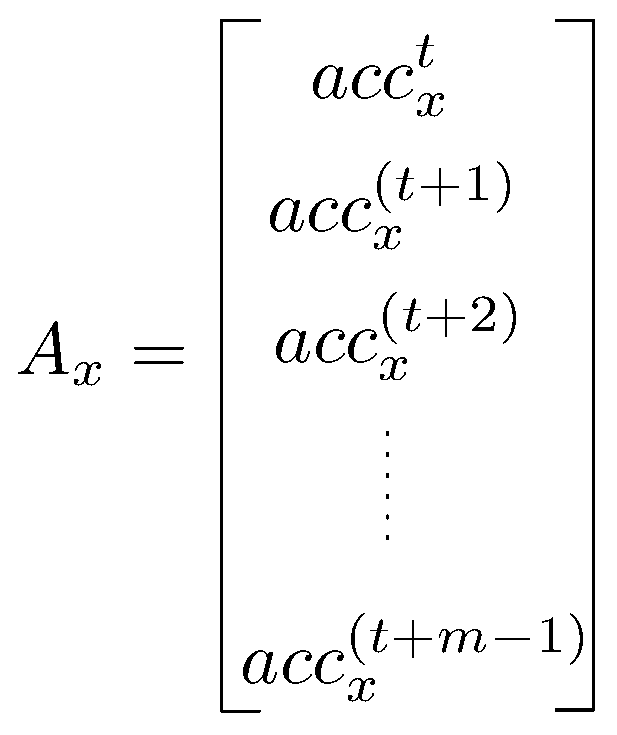
\includegraphics[width=0.22\textwidth]{figures/featureVectorNormal}    % The printed column width is 8.4 cm.
\caption{One of the features (accelerometer x-axis) of the original feature matrix (given in Fig.~\ref{fig:featureMatrix}) before adding extra features} 
\label{fig:featureVectorNormal}
\end{center}
\end{figure}

\begin{figure}[H]
\begin{center}
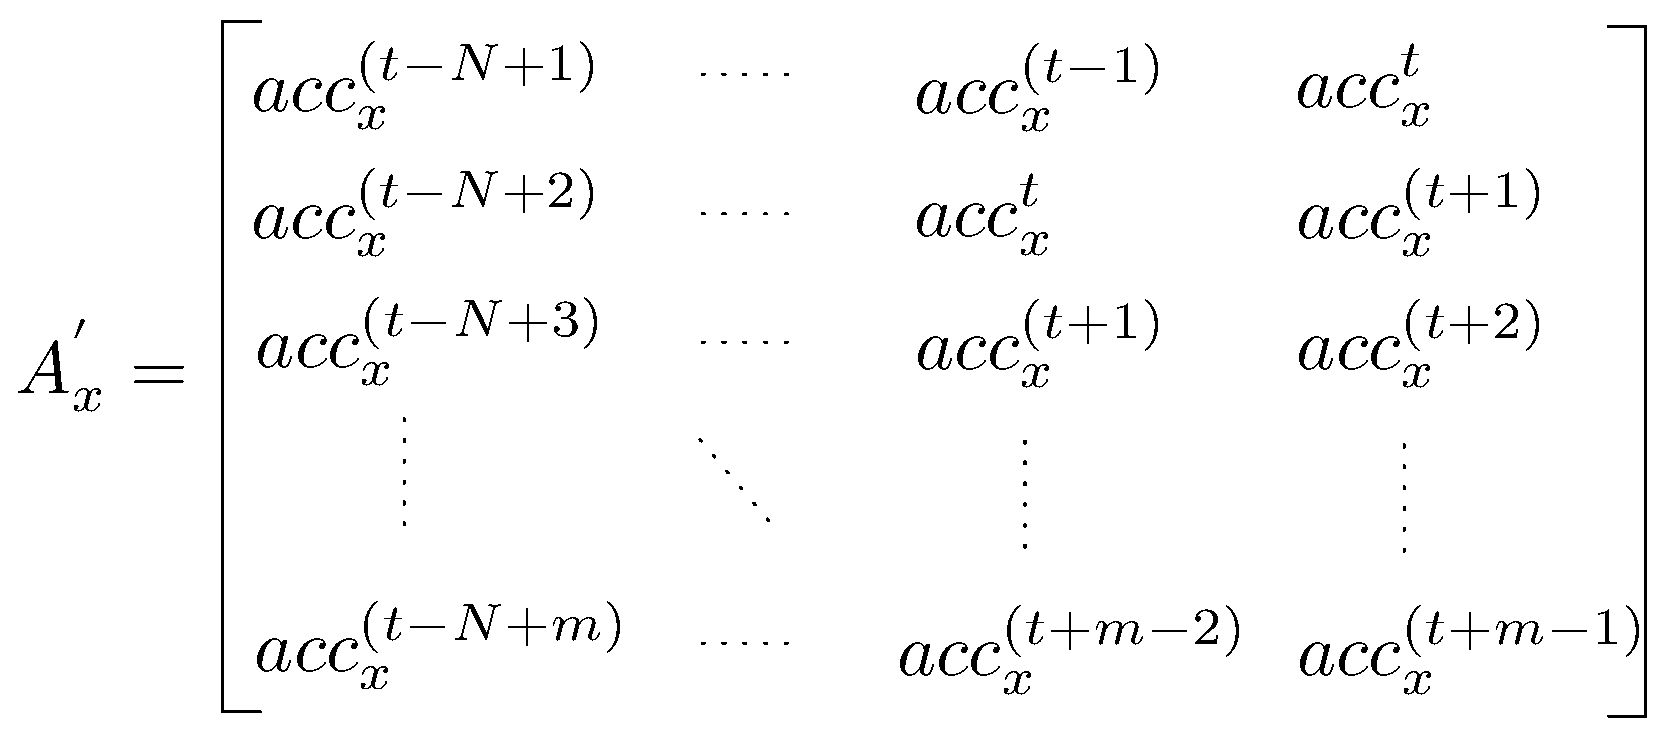
\includegraphics[width=0.63\textwidth]{figures/addingFeatures}    % The printed column width is 8.4 cm.
\caption{Addition of features to involve $N-1$ previous measurements} 
\label{fig:addingFeatures}
\end{center}
\end{figure}

Finally, this feature addition is applied to all features of the original feature matrix, resulting in $\bm{X'} \in {\rm I\!R^{m \times 6N}}$ :

\begin{equation}
\bm{X^{'}}= \begin{bmatrix} \bm{A}_x^{'}\ \bm{A}_y^{'} \ \bm{A}_z^{'} \ \bm{G}_x^{'} \ \bm{G}_y^{'} \ \bm{G}_z^{'}  \end{bmatrix}^{\rm T}
\end{equation}

where $\bm{A}_y^{'}$, $\bm{A}_z^{'}$, $\bm{G}_x^{'}$, $\bm{G}_y^{'}$, $\bm{G}_z^{'}$ is constructed in the same way as  $\bm{A}_x^{'}$ detailed in Fig.~\ref{fig:addingFeatures}.
The number of features have been increased to 24 in Table~\ref{tab:contSurfStuckAddedFeat}, which means only 3 previous measures for each different attribute have been added to the feature set ((3 past + 1 instant) * 6 axis).
This addition to the feature set, in general, deteriorated the performance of the classifier, especially the classifier with an untuned Gaussian kernel (\emph{f1Score}= $0.4167$) ($\Delta f1Score = -0.5135$). 
For the classifiers with tuned Gaussian kernels, \emph{f1Score} decreases by a small amount for the classifier tuned with heuristic method (\emph{f1Score} $= 0.9444$) and increases by an even smaller amount(\emph{f1Score} $= 0.9143$) hence the effect is not really obvious. 


% For tables use
\begin{table*}[h]
	\centering
% table caption is above the table
\caption{Untuned and tuned via heuristic approach and tuned via Bayesian optimization SVM classification evaluations}
\label{tab:contSurfStuckAddedFeat}       % Give a unique label
% For LaTeX tables use
\begin{tabular}{p{2.6cm}p{2cm}p{2.5cm}p{2.7cm}}
\hline\noalign{\smallskip}
 & Untuned \ 24 features & Tuned Heuristic 24 features & Tuned Bayesian Opt. 24 features\\
\noalign{\smallskip}\hline\noalign{\smallskip}
kernel scale & 1 & 6.0609 & 67.33 \\
box constraint & 1 & 10 &  47330\\
margin & 1.9733 & 3.6353 & 5.6484 \\
edge & 1.9678 & 3.6317 & 5.6404 \\
kFoldLoss & 5.6 x $10^{-3}$ & 3.44 x $10^{-4}$ & 6.19 x $10^{-4}$ \\
precision & 1 & 1 & 1 \\
recall & 0.2632 & 0.8947 & 0.8421\\
\textbf{f1Score} & 0.4167 & 0.9444 & 0.9143 \\
comp. time & 12.4s & 5581.9s &1205.2s \\
\noalign{\smallskip}\hline
\end{tabular}
\end{table*}

% Second trial for the same number of features
% For tables use
\begin{sidewaystable*}
	\centering
% table caption is above the table
\caption{Untuned and tuned via heuristic approach and tuned via Bayesian optimization SVM classification evaluations}
\label{tab:contSurfStuckAddedFeatDiffPercentage}       % Give a unique label
% For LaTeX tables use
\begin{tabular}{p{1.5cm}p{2cm}p{2.3cm}p{2.3cm}p{2.3cm}p{2.3cm}p{2.4cm}}
\hline\noalign{\smallskip}
 & Untuned  24 features & Tuned Heuristic 24 features & Tuned Bayesian 24 features & Untuned Heuristic 24 features \%60 test/training & Tuned Heuristic 24 features \%60 test/training & Tuned Bayesian 24 features \%60 test/training\\
\noalign{\smallskip}\hline\noalign{\smallskip}
kernel scale & 1 & 5.5154 & 24.9026 & 1 & 4.7577 & 24.9769\\
box constraint & 1 & 10 & 9172.9 & 1 & 10 & 85.3263\\
margin & 1.9697 & 4.0001 & 5.8651& 1.9685 & 3.7267 & 4.7728\\
edge & 1.9680 & 3.99 & 5.8651 & 1.9691 & 3.7270 & 4.7734\\
kFoldLoss & 5.5 x $10^{-3}$ & 4.8 x $10^{-4}$ & 6.8 x $10^{-4}$ & 5.4 x $10^{-3}$ & 5.5 x $10^{-4}$ & 7.3421 x $10^{-4}$\\
precision & 1 & 1 & 1 & 1 & 1 & 0.92\\
recall & 0.1739 & 1 & 1 & 0.22 & 0.96 & 0.92\\
\textbf{f1Score} & 0.2963 & 1 & 1 & 0.3607 & 0.9796 & 0.92\\
comp. time & 11.3s & 5853.3s & 1061s & 8.5s & 2924.3s & 235.671s\\
\noalign{\smallskip}\hline
\end{tabular}
\end{sidewaystable*}


Table~\ref{tab:contSurfStuckAddedFeat} and first 3 columns of Table~\ref{tab:contSurfStuckAddedFeatDiffPercentage} are the results of the same algorithm with same number of features and percentage of training/test set ratio. 
Due to usage of random functions, the seed value has been set to a constant value for reproducibility. 
Stratified sampling has been implemented to assure fair amount of data from both classes in both sets (training and test). 
Finally, it has been discovered that even with the selection of same number of data for the training and test sets for both classes (faulty and nominal), some combinations of possible training/test set selections result in more precise classifiers than others. 
This can be seen by observing the tuned \emph{f1Scores} (\emph{f1Scores}=$0.9444$ in and \emph{f1Score}$=0.9143$) in Table~\ref{tab:contSurfStuckAddedFeat} increasing to the \emph{f1Score} (\emph{f1Score}$=1$) in Table~\ref{tab:contSurfStuckAddedFeatDiffPercentage}.


Table~\ref{tab:contSurfStuckAddedFeatDiffPercentage} shows the evaluation results of SVM classifiers trained with different percentage of training and test sets. 
First 3 columns present the results for a test to training set ratio of $1/4$ while the last 3 columns present the ratio of $2/3$. \emph{f1Score} trained and tuned with $\%80$ training data implies that this percentage is a good choice for this problem (with an \emph{f1Score} of 1 for tuned classifiers). 

\iffalse

\begin{figure}
\begin{center}
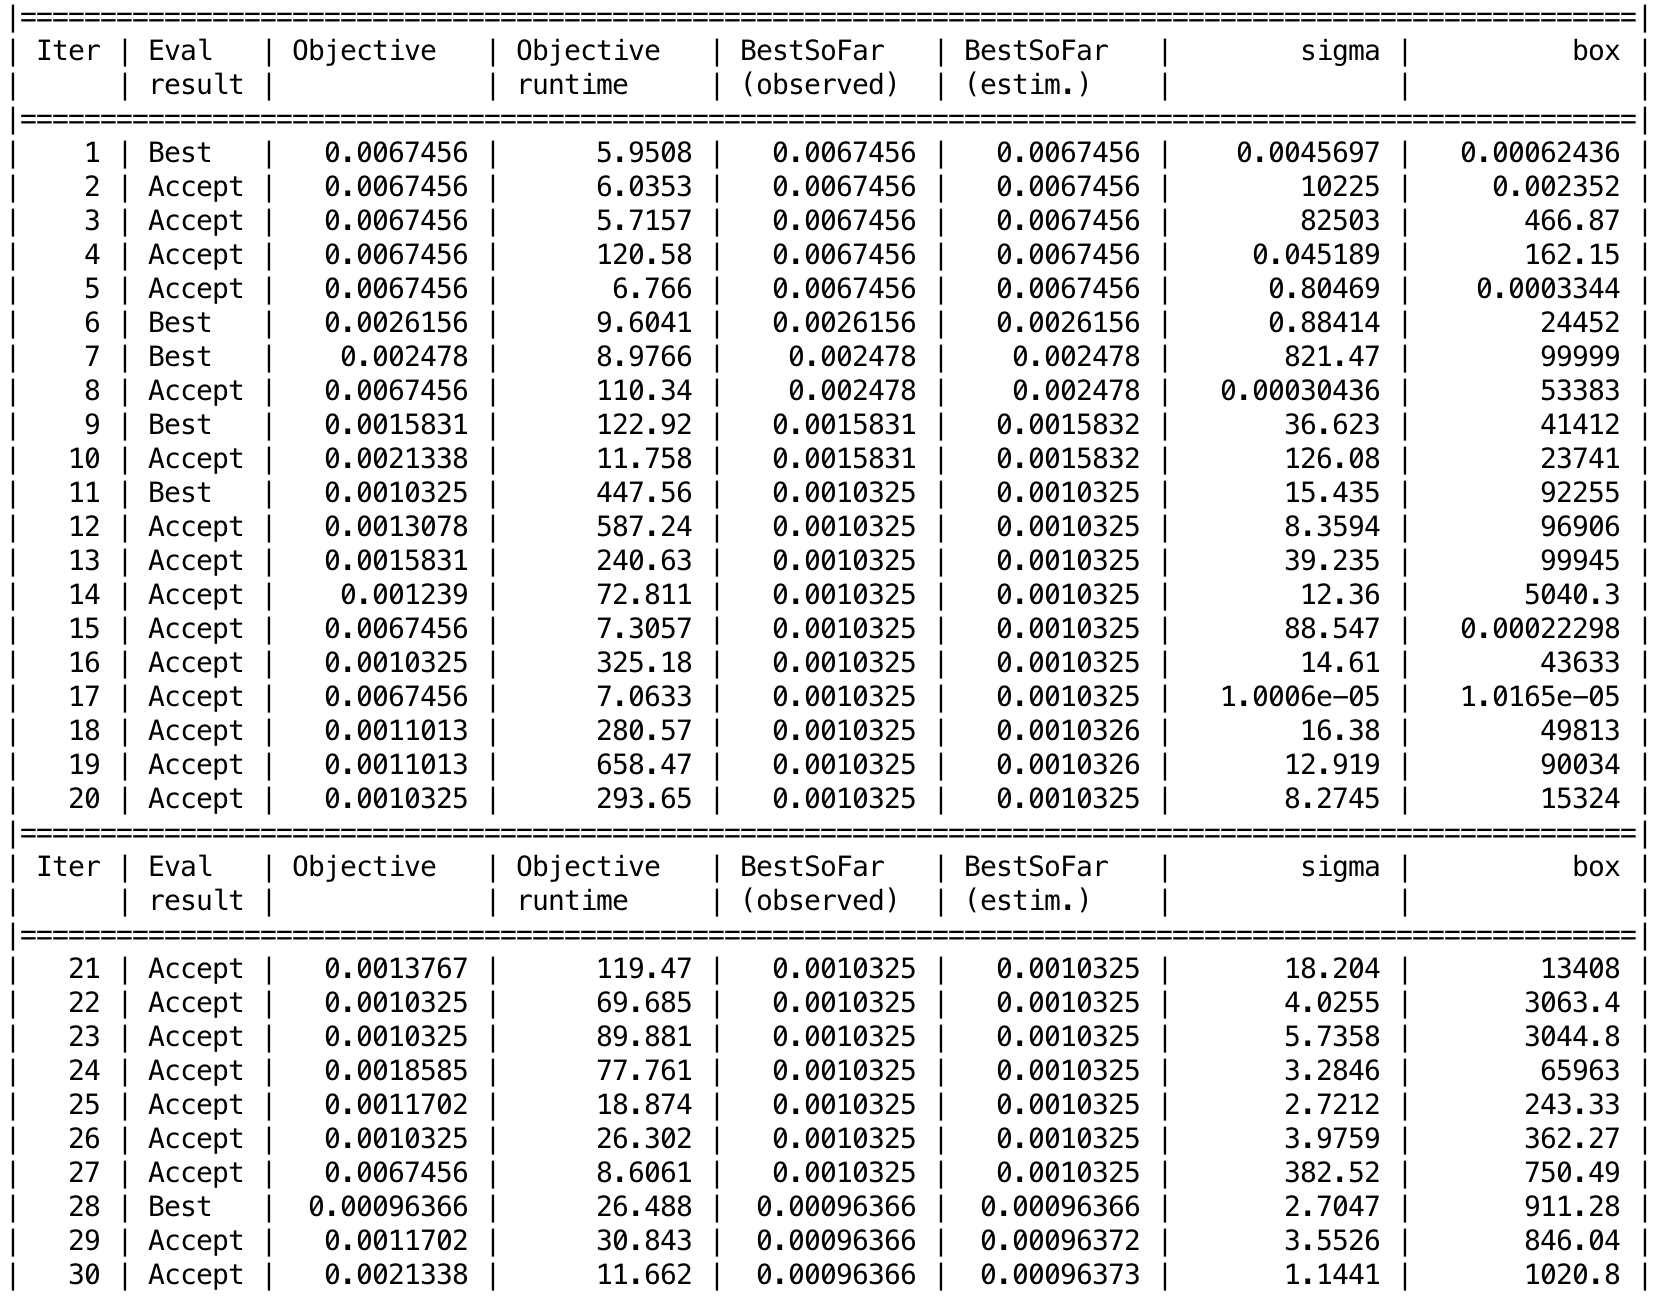
\includegraphics[width=15cm]{figures/optimizationSummaryStuckFault}    % The printed column width is 8.4 cm.
\caption{Optimization summary} 
\label{fig:optimizationSummaryStuckFault}
\end{center}
\end{figure}

\begin{figure}
\begin{center}
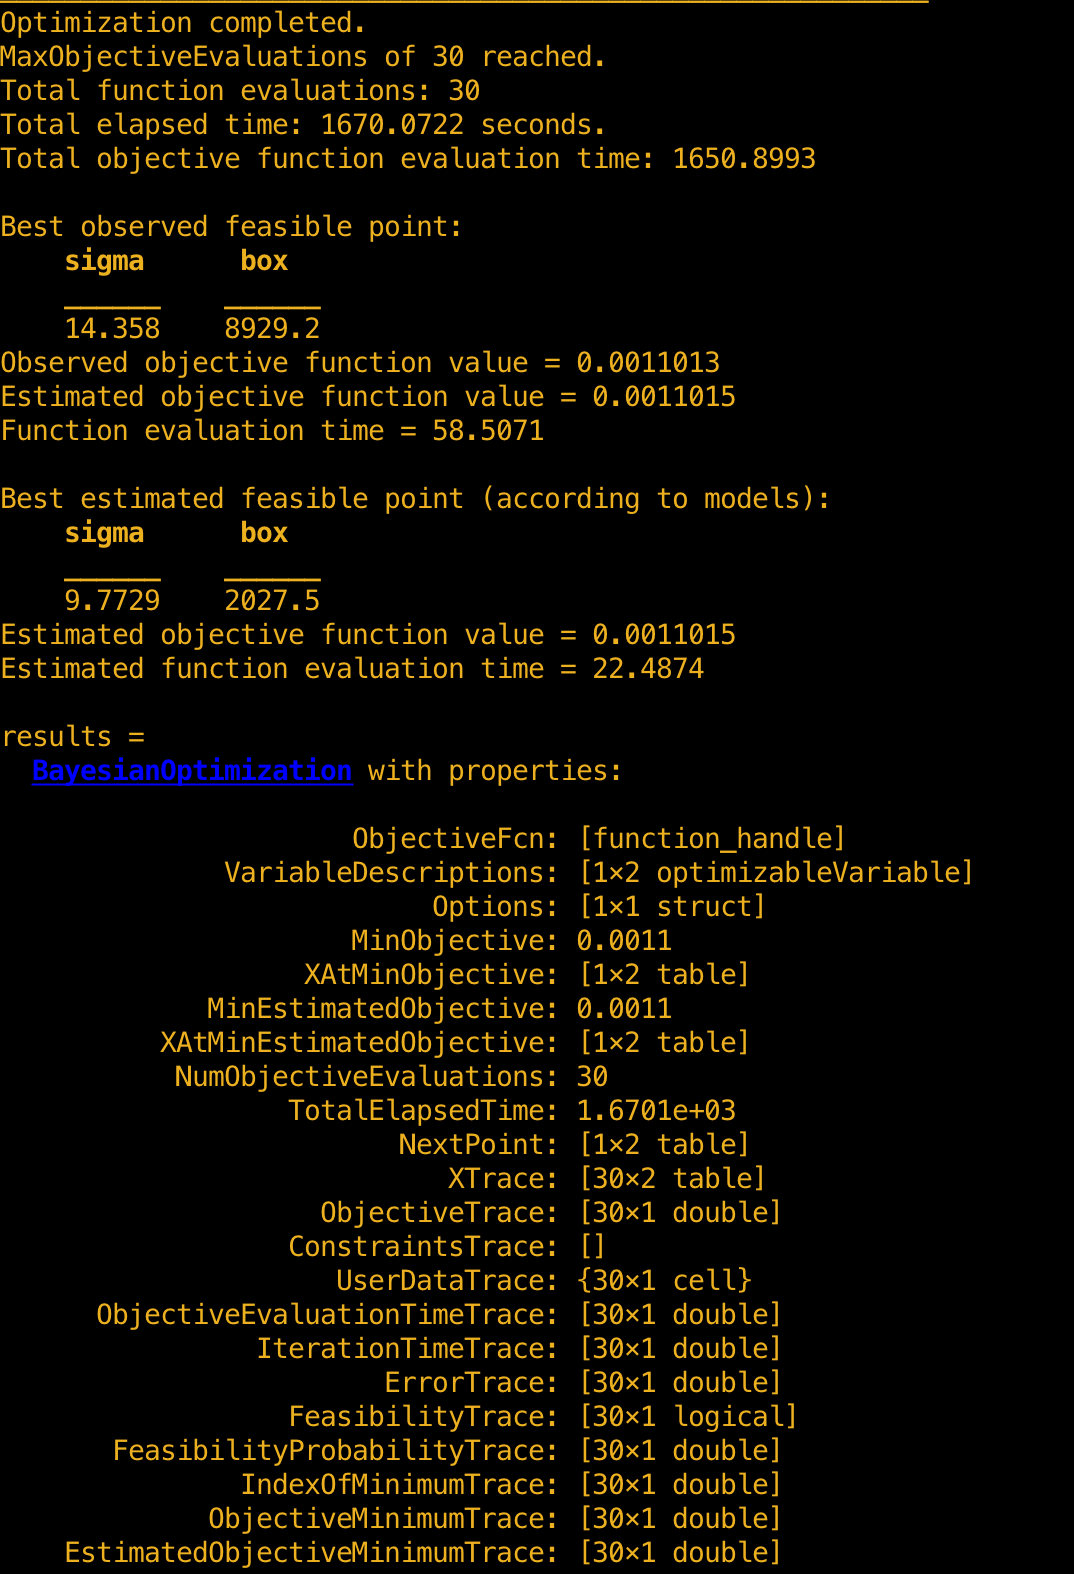
\includegraphics[width=15cm]{figures/optimizationResultsStuckFault}    % The printed column width is 8.4 cm.
\caption{Optimization results} 
\label{fig:optimizationResultsStuckFault}
\end{center}
\end{figure}

\begin{figure}
\begin{center}
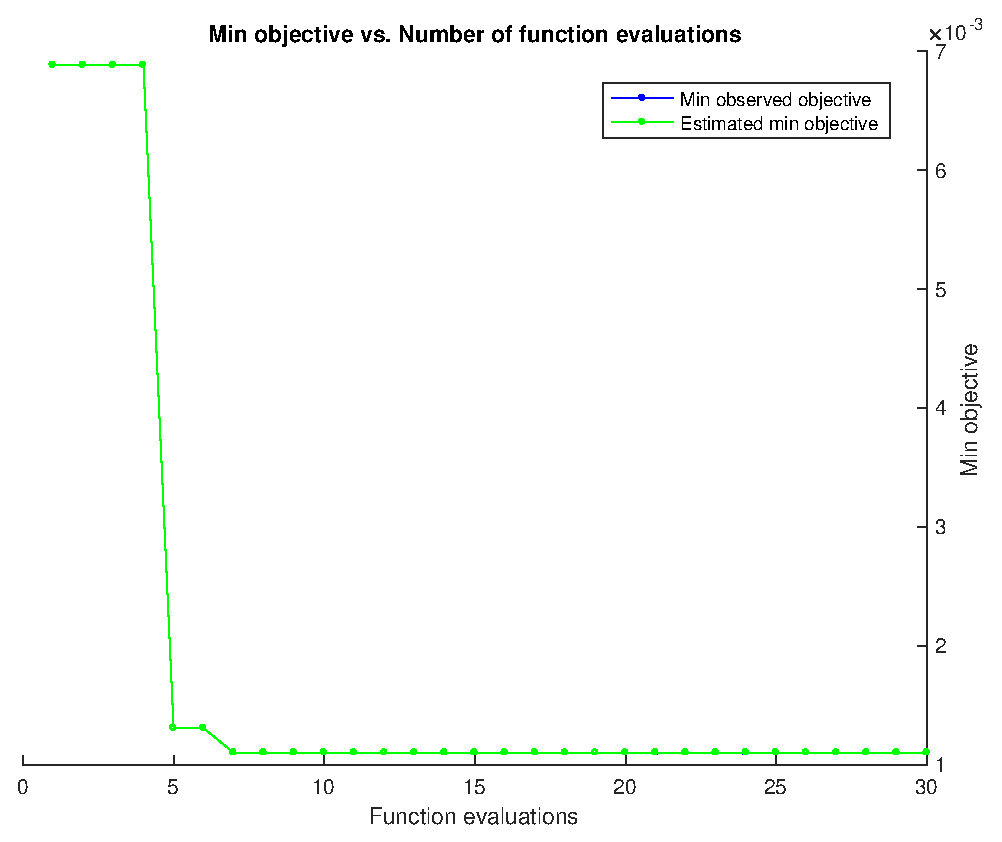
\includegraphics[width=11cm]{figures/funcEval2}    % The printed column width is 8.4 cm.
\caption{Function evaluations during optimization} 
\label{fig:funcEval1}
\end{center}
\end{figure}

\begin{figure}
\begin{center}
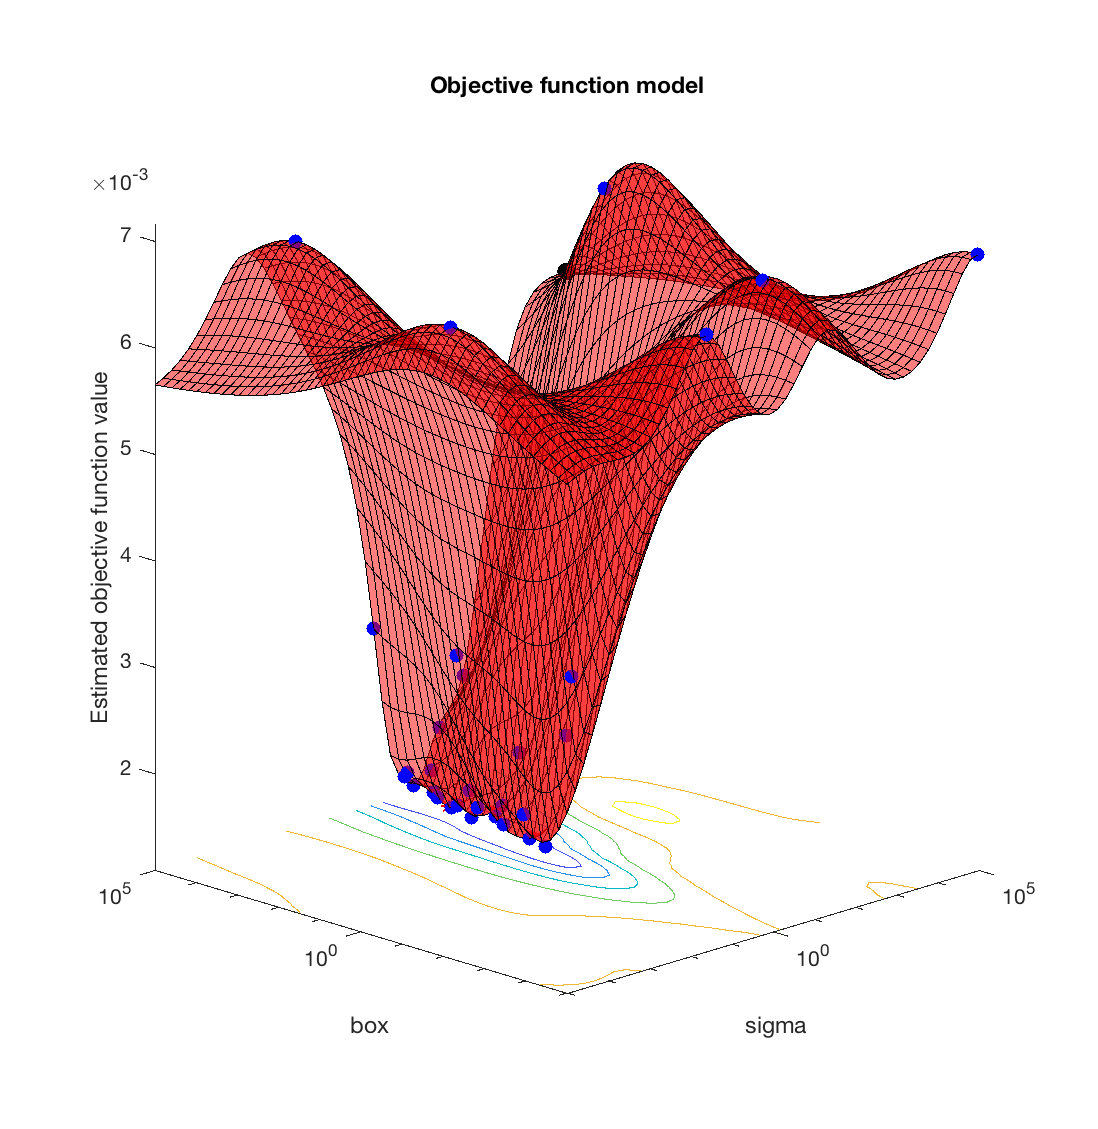
\includegraphics[width=11cm]{figures/objFunc2}    % The printed column width is 8.4 cm.
\caption{Objective function for different box parameter and sigma values} 
\label{fig:objFunc1}
\end{center}
\end{figure}

\fi

\subsection{Control surface loss of efficiency fault}


Loss of efficiency fault was generally more difficult to diagnose. 
First, a fault of \%10 loss of efficiency on the left elevon has been investigated (SETTINGS 1.0 0.9 0.0 0.0). 
This fault was the first injected fault in the course of the flight so the corresponding nominal phase is quite long. 
During those first minutes of the flight, the nominal mode kept quite long to gather more nominal data from the flight before initiating the fault sequences. 
The results showed the insufficiency of the method to diagnose the fault (see Table~\ref{tab:loe10_40} noted as LOE1) even with a Gaussian kernel which resulted in exceptional results for stuck control surface diagnostics. 
One of the explanations for that might be, since the control surfaces is not moving in a wide range during the nominal course of action, \%10 degradation in the movement of the elevon does not really change the dynamic behavior of the drone yet not easy to pinpoint from the measurements.
Another reason, likely to be the main driver, could be the compensation of the fault via the controller.
The aim of the controller onboard is to minimize the error to track a given reference trajectory and corresponding attitude references. 
Hence, when this error is not minimized, for one reason or another, the controller re-computes the control signal to minimize this error. 
So either an error due to a different wind condition or a fault in the control surface, the controller's duty is to minimize this error, so a well designed controller might handle that especially for the condition where the effect of disturbance is not catastrophic. 
This controller's compensation for the fault could be known by observing output of the controller and feeding this information as well in the set of instances. 
But, during the course of this study, the abilities of a classifier without the information from the controller is investigated. 
The main reason behind is to challenge the abilities of a small and cheap set of health monitoring system that does not rely on the information from the autopilot. 

The loss of efficiency of the left elevon is increased to \%40 degradation to investigate if this time the SVM classifier will be able to classify the fault. This fault is coined as LOE2 in the Table~\ref{tab:loe10_40}. The results show no recuperation in the classification results for neither untuned nor tuned classifiers with \emph{f1Score}$=0.0032$ and \emph{f1Score}$=0.2$ respectively.


% For tables use
\begin{table*}
% table caption is above the table
\caption{\%10 and \%40 Loss of efficiency fault in left elevon classification results with Gaussian kernel}
\label{tab:loe10_40}       % Give a unique label
% For LaTeX tables use
\begin{tabular}{p{1.65cm}p{2cm}p{2cm}p{2cm}p{2cm}p{2cm}p{2cm}}
\hline\noalign{\smallskip}
 & Untuned LOE1 & Tuned Heuristic LOE1 & Tuned Bayesian Opt. LOE1& Untuned LOE2 & Tuned Heuristic LOE2 & Tuned Bayesian Opt. LOE2\\
\noalign{\smallskip}\hline\noalign{\smallskip}
\textbf{f1Score} & NaN & 0.1235 & 0.0111 & 0.2716 & 0.2756 & NaN\\
kFoldLoss & 5.32 x $10^{-2}$ &  5.19 x $10^{-2} $&  5.33 x $10^{-2}$ & 3.84 x $10^{-2}$ &  3.7 x $10^{-2} $&  5.33 x $10^{-2}$ \\
precision & 1 & 0.66 & NaN & 1 & 0.66 & NaN\\
recall & 0.0016 & 0.119 & 0  & 0.0016 & 0.119 & 0 \\
\noalign{\smallskip}\hline
\end{tabular}
\end{table*}	


% For tables use
\begin{table*}
	\centering
% table caption is above the table
\caption{\%40 Loss of efficiency fault in both elevon classification results with Gaussian kernel for two different number of nominal data sets}
\label{tab:loe40_decreasedNumNomMeas}       % Give a unique label
% For LaTeX tables use
\begin{tabular}{p{1.65cm}p{2cm}p{2cm}p{2cm}p{2.2cm}p{2.2cm}p{2.2cm}}
\hline\noalign{\smallskip}
 & Untuned & Tuned Heuristic  & Tuned Bayesian Opt. & Untuned& Tuned Heuristic  & Tuned Bayesian Opt. \\
 & $\sim$15min & $\sim$15min & $\sim$15min &  $\sim$3min & $\sim$3min & $\sim$3min\\
\noalign{\smallskip}\hline\noalign{\smallskip}
\textbf{f1Score} & NaN & 0.1235 & 0.0111 & 0.2712 & 0.2756 & NaN\\
kFoldLoss & 4.76 x $10^{-2}$ &  4.62 x $10^{-2} $&  4.73 x $10^{-2}$ & 19.01 x $10^{-2}$ &  18.87 x $10^{-2} $&  20.61 x $10^{-2}$ \\
precision & NaN & 0.66 & 0.27 & 0.7109 & 0.6992 & NaN\\
recall & 0 & 0.0681 & 0.0057  & 0.1679 & 0.1716 & 0 \\
\noalign{\smallskip}\hline
\end{tabular}
\end{table*}

Since the results were very poor in terms of classifying faults, the faults have been increased to have \%40 degradation in both elevon. 
The idea is to see at which level the result of classification will improve and also to search for any reasons behind this ineffectiveness except controller's compensation. 
Another issue to investigate was the effect of number of instances for the larger datasets (nominal class) to classification. 
For that purpose, three different size for nominal data set ($\sim$15min, $\sim$6min, $\sim$3min) was investigated in terms of their effects to classification performance for a faulty measurement data set of $\sim$1min. 
Classification results for two of the situations ($\sim$15min, $\sim$3min) are given in Table~\ref{tab:loe40_decreasedNumNomMeas}. 
The reduction of the nominal data set was not random selection throughout the complete set, but only the last part of the nominal data set that is closer to the faulty data in terms of flight time instance was selected. 
The first simulation involved $\sim$15min nominal measurements, hence the most skewed classification. 
An untuned SVM classifier with a Gaussian kernel was not able to classify (\emph{f1Score}$ = NaN$) the fault. 
Even when tuned, the classification performance was too poor to be used for predicting faults (\emph{f1Score}$ = 0.12$) as shown in Table~\ref{tab:loe40_decreasedNumNomMeas}. 
Reducing the number of the larger class, gyro and accelerometer measurements during nominal phase, an untuned SVM classifier with Gaussian kernel still results poorly in classification (\emph{f1Score}$ = 0.0073$) and tuning does not help much (\emph{f1Score}$ = 0.13$). 
Compared to the larger nominal class measurements case, it gives the idea that reducing the number of instances of the bigger class might help to improve classification performance ($\Delta f1Score = 0.01$).
A further reduction in the number of instances of the nominal class ($\sim$3min) still gives poor classification results with an untuned SVM classifier with a Gaussian kernel (\emph{f1Score} $= 0.2712$) although an improvement observed compared to the wider nominal data set ($\Delta f1Score = 0.2616$). 
Tuning the classifier did not enhance the classification result noticeably (\emph{f1Score} $= 0.2756$).


% For tables use
\begin{table*}
	\centering
% table caption is above the table
\caption{\%40 Loss of efficiency fault in left elevon classification results with Gaussian kernel for 24 - 120 - 300 features cases}
\label{tab:loe40_featureAddition}       % Give a unique label
% For LaTeX tables use
\begin{tabular}{l m{1.6cm} m{1.6 cm} m{1.6 cm} m{1.6 cm} m{1.6 cm} m{1.6 cm}}
\hline\noalign{\smallskip}
 & Untuned & Tuned Heuristic  & Untuned & Tuned Heuristic  & Untuned & Tuned Heuristic \\
 & 24 & 24 & 120 & 120 &  300 &  300 \\
\noalign{\smallskip}\hline\noalign{\smallskip}
\textbf{f1Score} & 0.1375 & 0.6414 & NaN & 0.9635 & NaN & 0.9896\\
kFoldLoss & 0.1898 & 0.1194 &  0.2075 & 0.0308 & 0.2071 & 0.0091\\
precision & 0.9545 & 0.7254 & NaN & 0.9804 & NaN & 0.9981\\
recall & 0.0741 & 0.5732 & 0 & 0.9471 & 0 & 0.9812 \\
\noalign{\smallskip}\hline
\end{tabular}
\end{table*}


Since reducing the number of instances of the larger class (nominal phase measurements) in the classification does help but not result in satisfactory results for classification, adding new attributes to the feature set is considered. 
For that, the previous measurements of the same attribute is added to the input matrix to have the time dependent change in the behavior of the observed physical variable. Results for a set of total number of 24, 100 and 300 features has been given in Table~\ref{tab:loe40_featureAddition}. 
To start with the discussion of the effect of adding previous measurements as separate features to the feature set, previous 3 measurements have been added to the input data set, resulting in 4 x 6 = 24 features. 
Adding 3 previous instance in time for each sensor measurement decreased the performance of the untuned classifier with a Gaussian kernel \emph{f1Score} $= 0.1375$ which is an classification performance decrease of $\Delta f1Score = 0.1341$. 
Adding more features the classifier still not able to classify when untuned but by tuning the \emph{f1Score} can be improved heavily producing a classifier with an \emph{f1Score} of 0.9635 for 120 feature case and can be even more fined to a \emph{f1Score} of 0.9896 for 300 features in total.
 So adding features advances the classification but only with proper tuning is achieved. Otherwise, untuned, the results are even worse than before adding features.


\subsection{Use of spinors as attributes}
In this thesis, until now, use of feature engineering to ameliorate the classification performance has been performed mainly utilizing the addition of new features to include previous measurements in all instances. The idea was to include the time evolution of the signal as well as the instantaneous measurements in the instances. Here another idea has been applied as feature engineering: to replace angular velocity measurements from gyros with spinors such that feature matrix is given as in Fig.~\ref{fig:featureMatrixSpinors}. For that, the kinematics equation, presented here again as a reminder, has to be solved numerically to attain quaternions from angular velocities.

\begin{figure}[h]
\begin{center}
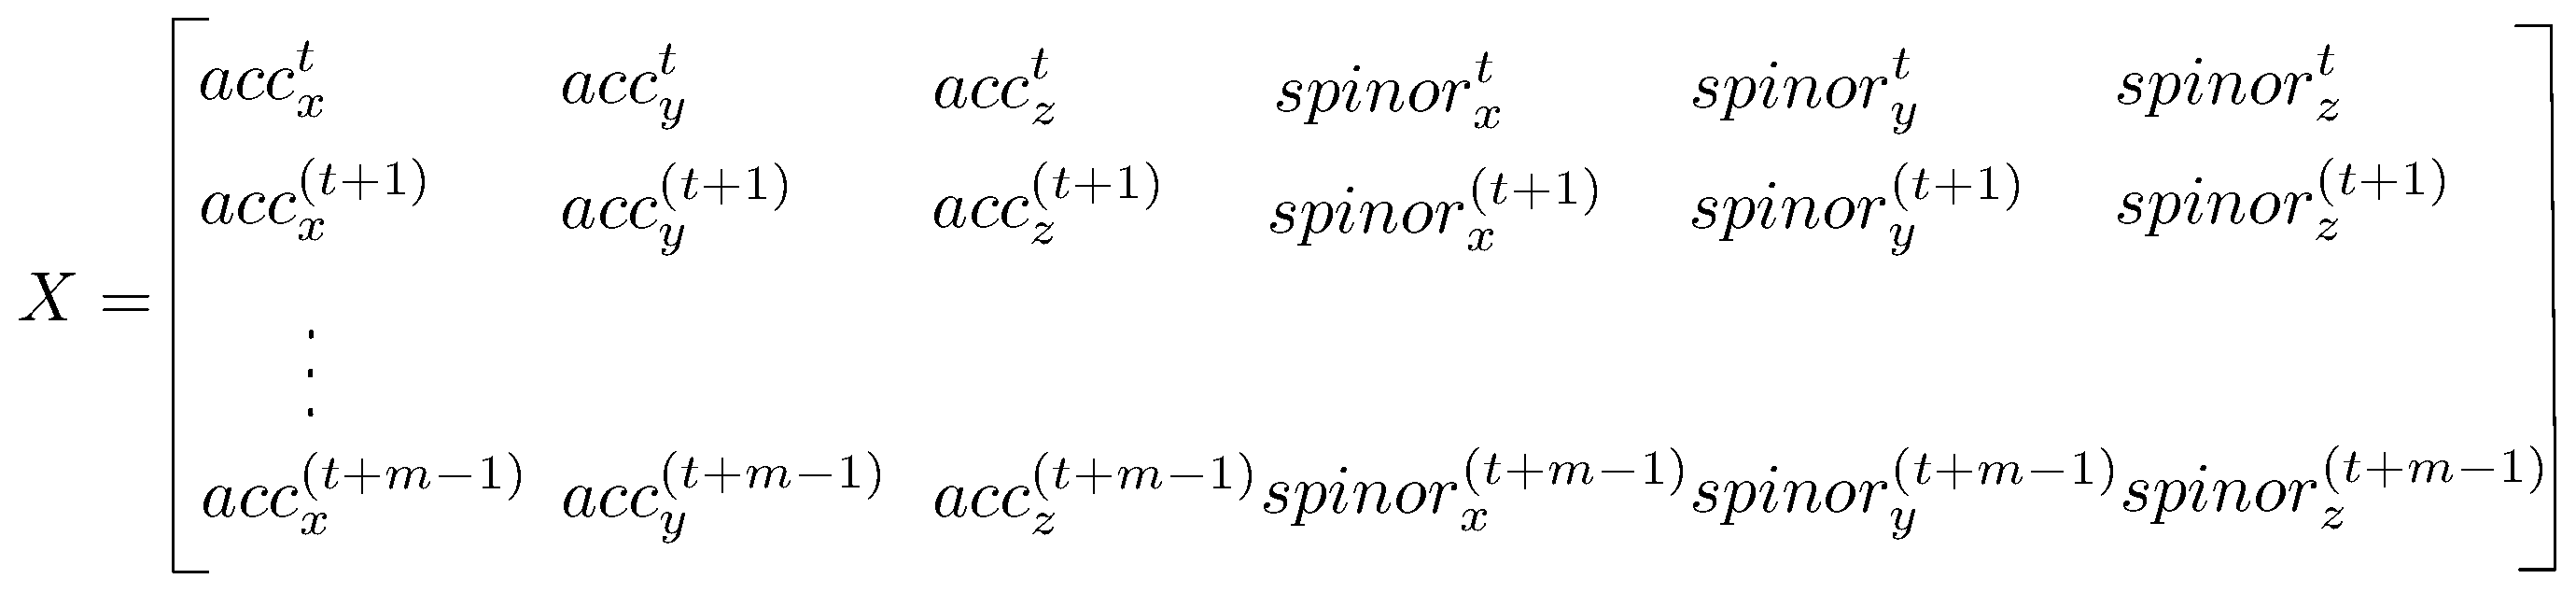
\includegraphics[width=13cm]{figures/featureMatrixSpinors}    % The printed column width is 8.4 cm.
\caption{New feature matrix when spinors are used as features rather than gyro measurement} 
\label{fig:featureMatrixSpinors}
\end{center}
\end{figure}

For that, kinematics equations Eq. \ref{eqn:angVelocityKinematics} have been solved numerically.

\begin{align}{\label{eqn:angVelocityKinematics}}
\begin{split}
 \dot{q}_0 &= -\frac{1}{2} \bm{q}_\nu^T \bm{\omega}\\
 \dot{\bm{q}}_\nu &= \frac{1}{2}\Big(\bm{q}_\nu^\times + q_0 \bm{I}_3 \Big) \bm{\omega} \\
\end{split}
\end{align}

\begin{equation}{\label{quaternionDefinition}}
\bm{q} = \begin{bmatrix} 
cos\Big(\frac{\theta}{2}\Big) & sin(\frac{\theta}{2}) \bm{e} \\
\end{bmatrix}
\end{equation}

Given the quaternion definition in  Eq. \ref{quaternionDefinition} 

\begin{equation}{\label{spinorDefinition}}
log(\bm{q}) = \begin{bmatrix} 
0 & \frac{\theta}{2} \bm{e} \\
\end{bmatrix}
\end{equation}

spinor are calculated with taking the logarithm of quaternion described as in Eq. \ref{spinorDefinition}.

\begin{table}[hbt!]
\caption{\label{tab:spinorsGaussian} Results for untuned, tuned SVM classifiers with spinors as attributes}
\centering
\begin{tabular}{lcccc}
\hline
%& Transition& & \multicolumn{2}{c}{}\\\cline{2-2}
& \makecell{Untuned \\ Gaussian kernel} & \makecell{Untuned \\ linear kernel} & \makecell{Tuned heuristic \\ Gaussian kernel}& \makecell{Tuned Bayesian \\ Gaussian Kernel}\\\hline
f1Score& 0.9555 & 0.6878 & 0.9795 & 0.9915\\
kFoldLoss & 0.0213 & 0.1047 & 0.0098 & 0037 \\
precision& 0.9618 & 0.9758 & 0.9704 & 0.9925\\
recall& 0.9492 & 0.5311 & 0.9887 & 0.9906\\
boxConstraint& 1 & 1 & $10^{5}$ & 9.6 x $10^{4}$ \\
kernelScale& 1 & 1 & 5.6611 & 3.8346 \\
compTime & 5.17s& 5.47s &11470.03s& 11373.91\\
\hline
\end{tabular}
\end{table}

Result given in Table~\ref{tab:spinorsGaussian} shows an apparent increase in classification with \emph{f1Score} reaching up to 0.9915.

\subsubsection{Untuned classification superiority}

The first promising result by using spinors for classification is its advantage in untuned classifiers. This can be seen by checking from Table~\ref{tab:GaussianUntuned} the \emph{f1Score} of the SVM classifier without tuning. As mentioned before, untuned classifier for added features results poorly although increasing the classification accuracy when tuned properly. Untuned SVM classifier with spinors as attributes results in an increased classification performance with an \emph{f1Score} of 0.6878. Using a Gaussian Kernel which is mathematically represented as in Eq. \ref{eqn:gaussianKernel}, \emph{f1Score} even increases up to 0.9555.

\begin{equation}{\label{eqn:gaussianKernel}}
K (x,z) = exp \bigg(-\frac{\Vert x - z \Vert ^ 2}{2 \sigma^2} \bigg)
\end{equation}


\begin{table}[hbt!]
\caption{\label{tab:GaussianUntuned} Results for untuned SVM classifiers with added features, original features and spinors as attributes}
\centering
\begin{tabular}{lccccc}
\hline
%& Transition& & \multicolumn{2}{c}{}\\\cline{2-2}
& \makecell{Untuned \\ Gaussian kernel \\ 300 feat.} & \makecell{Untuned \\ Gaussian kernel \\ 24 feat.} & \makecell{Untuned \\ Gaussian kernel \\ original feat.} & \makecell{Untuned \\ Linear kernel \\ spinors}& \makecell{Untuned \\ Gaussian kernel \\ spinors }\\\hline
f1Score& NaN & 0.1375 & 0.2712 & 0.6878 & 0.9555\\
\hline
\end{tabular}
\end{table}

\subsubsection{Tuned classification Bayesian optimization efficiency}

Table~\ref{tab:GaussianTuned} shows the results except the simulations using spinors, the heuristic optimization gives a better performance for tuning the classifier while the Bayesian optimization is likely to converge to a local minima. But when spinors used, Bayesian optimization results in a better performance in tuning the classifier as shown under Table~\ref{tab:GaussianTuned} in Tuned Gaussian Kernel spinors row.  

\begin{table}[hbt!]
\caption{\label{tab:GaussianTuned} Results for tuned SVM classifiers with added features, original features and spinors as attributes}
\centering
\begin{tabular}{lcc}
\hline
%& Transition& & \multicolumn{2}{c}{}\\\cline{2-2}
& \makecell{ Heuristic\\ tuning} & \makecell{ Bayesian\\ tuning}\\\hline
 \makecell{Tuned Gaussian kernel \\ 300 feat.} & 0.98 & 0.92 \\
 \makecell{Tuned Gaussian kernel \\ 24 feat.} & 0.64 & 0.35 \\
 \makecell{Tuned Gaussian kernel \\ original feat.}  & 0.2756 & NaN\\
  \makecell{Tuned Gaussian kernel \\ spinors} & 0.97 & 0.99 \\
\hline
\end{tabular}
\end{table}

\section{Conclusion}

In this chapter, we focus on the results of SVM classification application to Fault Detection \& Diagnosis problem. Fault classification simulations are explained under two main sections: classification of faults based on simulated flight measurements and classification of faults based on real flight data. 

First part of this chapter gives the results of SVM classification on data generated from simulations. 
To simulate the data, equations of motions given in \emph{Nonlinear Aircraft Model} has been numerically solved for the states. 
Then sensor measurements (accelerometer and gyro data) have been calculated using the states and the specifications of the sensors. 
Generated data is usually more structured compared to the real flight data. 
In this preliminary application of SVM to fault diagnosis, we aimed to start with an easier problem, and used data generated from models.
There is no controller involved in the model in this preliminary application of SVM to detection to discard the controller's effect on the diagnosis. 

The second part investigates the fault detection with real flight data. 
SVM, being a supervised learning algorithm, requires labeled data for both nominal and faulty flight conditions. 
So faulty flights were realized with a security pilot ready to recover in loss of control of the aircraft.
For the faulty flight data gathering, some modifications to the \emph{Paparazzi} autopilot was necessary in two main parts: Injecting the faults real-time from GCS, and editing the controller onboard so that the sent faulty input values configures the servos as manipulated from the GCS. 

With the flight data, two main classes of faults, control surface stuck and loss of effectiveness, have been investigated separately. 
A variety of techniques implemented to improve the performance of the classification such as feature engineering and tuning the classifiers. 
